\documentclass[a4paper, 11pt]{article}
%\documentclass[a4paper, 11pt]{exam}


%%%%%%%%%%%%%%%%%%%%%%%%%%%%%%%%%
%	 PACKAGES	%
%%%%%%%%%%%%%%%%%%%%%%%%%%%%%%%%%
% Codierung von in und Output
\usepackage[utf8]{inputenc}
\usepackage[T1]{fontenc}

% AMS-Pakete für Mathe
\usepackage{amsthm,amssymb,amsmath}

% Sprachpaket neue rechtschreibung
\usepackage[ngerman]{babel} 


\usepackage[many]{tcolorbox}

%Header und Seitengrösse
\usepackage{fancyhdr}
\usepackage{geometry}

% Paket für Links im PDF (glaubs)!
\usepackage[hidelinks]{hyperref}

%Paket um ganze pdf-File zu importieren (Arbeitsblätter aus Analysis DMK)
\usepackage{pdfpages}

%TColorbox nutzt Theoreme und bessere Verweise
\tcbuselibrary{theorems}
\usepackage{cleveref}

%Package, um Aufgaben auf mehrere Spalten zu verteilen.
\usepackage{tasks}
\usepackage{multicol}

%Tikz
\usepackage{tikz}
\usetikzlibrary{matrix, positioning}
\usepackage{pgfplots}
\pgfplotsset{compat=1.18}




%Programmcode-Darstellung
\usepackage{listings}
\usepackage{xcolor}
\lstset{basicstyle=\ttfamily, language= Python}
\definecolor{codekeyword}{rgb}{0.11,0.53,0.63}
\definecolor{codenumbers}{rgb}{0.71,0.21,0.30}
\definecolor{codeoperation}{rgb}{0.57,0.32,0.59}
\definecolor{codecomment}{rgb}{0.17,0.59,0.28}
\definecolor{backcolour}{rgb}{0.98,0.97,0.99}
\definecolor{codestring}{rgb}{0.84,0.56,0.16}
\lstdefinestyle{mystyle}{
    backgroundcolor=\color{backcolour},   
    commentstyle=\color{codecomment},
    keywordstyle=\color{codekeyword},
    numberstyle=\tiny\color{black},
    stringstyle=\color{codestring},
    basicstyle=\ttfamily\footnotesize,
    breakatwhitespace=false,         
    breaklines=true,                 
    captionpos=b,                    
    keepspaces=true,                 
    numbers=left,                    
    numbersep=5pt,                  
    showspaces=false,                
    showstringspaces=false,
    showtabs=false,                  
    tabsize=4
}

\lstset{style=mystyle}







% kein Plan, was das folgende macht... :(
% \lstset{basicstyle=\ttfamily}
% \makeatletter
% \def\BState{\State\hskip-\ALG@thistlm}
% \makeatother

\usepackage{graphicx}
\usepackage{hyperref}
\usepackage{array}
\hypersetup{colorlinks=true}

% damit kann man nummerierte Liste unterbrechen und wieder aufnehmen
\usepackage{enumitem} 

%%%CHANGE LABEL FIGURE
\usepackage[figurename=Abbildung.]{caption}

%%%%%%%%%%%%%%%%%%%%%%%%%%%%%%%%
%%%%%%%%%%%	LAYOUT	%%%%%%%%%%%%
%%%%%%%%%%%%%%%%%%%%%%%%%%%%%%%%

\geometry{
	a4paper,
	total={165mm,225mm},
	left=25mm,
	top=35mm,
}

%keine Einrückung bei Absatz dafür Abstand
\setlength\parindent{0pt}
\setlength{\parskip}{1em}

%Header
\pagestyle{fancy}
\setlength{\headheight}{13.6pt}
\renewcommand{\sectionmark}[1]{ \markright{#1}{} }
\lhead[L]{M. Anderegg}
\chead{}
\rhead{Matrizen - \rightmark}
\lfoot{}
\cfoot{\thepage}
\rfoot{}





%%%%%%%%%%%%%%%%%%%%%%%%%%%%%%%%
%%%%%%%%% TCB-Commands %%%%%%%%%
%%%%%%%%%%%%%%%%%%%%%%%%%%%%%%%%

\newtcbtheorem
[auto counter, number within=section, crefname={beispiel}{beispiele}, Crefname={Beispiel}{Beispiele}] % Nummerierung und Name bei Verweis
{bsp} % Name der Umgebung \begin{bsp}
{Beispiel} %Name der im Titel angezeigt wird
{breakable, enhanced jigsaw, fonttitle=\bfseries, coltitle = black, colbacktitle = orange!15, righthand width=3cm,
	sharp corners,boxrule=.4pt,colback=orange!5} %%Optionen für die Box. 
	%Breakable und Enhanced lassen zu, dass sich die Box auf zwei Seiten verteilt.
{bsp} %So wird intern auf die Referenz verwiesen.

\newtcbtheorem[auto counter,  crefname={lernaufgabe}{lernaufgaben},
Crefname={Lernaufgabe}{Lernaufgaben}]{LA}{Lernaufgabe}{
	breakable, enhanced jigsaw, fonttitle=\bfseries, coltitle = black, colbacktitle = cyan!15, righthand width=3cm,
	sharp corners,boxrule=.4pt,colback=white}{LA}

\newtcbtheorem[auto counter, number within=section, Crefname={Übung}{Übungen}] {ueb}{Übung}{
	breakable, enhanced jigsaw, fonttitle=\bfseries, coltitle = black, colbacktitle = blue!15, righthand width=3cm,
	sharp corners,boxrule=.4pt,colback=blue!5}{uebng}


\newtcbtheorem[auto counter, number within=section, crefname={definition}{definitionen},
Crefname={Definition}{Definitionen}]{definition}{Definition}{
	breakable, enhanced jigsaw, colframe=green!70!black, fonttitle=\bfseries, coltitle = white, colbacktitle = green!70!black, enhanced, attach boxed title to top left={yshift=-0.1in, xshift=0.15in},}{def}

\newtcbtheorem[auto counter, number within=section, crefname={Satz}{Sätze},
Crefname={Satz}{Sätze}]{satz}{Satz}{%
	breakable, enhanced jigsaw, lower separated=false,
	colframe=red!70!white, fonttitle=\bfseries, coltitle = white, colbacktitle = red!70!white, enhanced, attach boxed title to top left={yshift=-0.1in,xshift=0.15in},
}{satz}




%%%%%%%%%%%%%%%%%%%%%%
%%%% Mathe-Befehle %%%
%%%%%%%%%%%%%%%%%%%%%%


\newcommand{\N}{\mathbb{N}}
\newcommand{\Z}{\mathbb{Z}}
\newcommand{\Q}{\mathbb{Q}}
\newcommand{\R}{\mathbb{R}}
\newcommand{\C}{\mathbb{C}}
\newcommand{\LL}{\mathbb{L}}
\newcommand{\DD}{\mathbb{D}}
\newcommand{\Ra}{\Rightarrow}



\begin{document}

\title{Lineare Abbildungen und Matrizen}
\author{M. Anderegg}
\date{} % sonst wird das Datum im Titel angezeigt
\maketitle 


\section{Lineare Abbildungen}
In diesem Abschnitt werden wir eine spezielle Art von geometrischen Abbildungen untersuchen. Dazu werden wir Punkte in der Ebene oder im dreidimensionalen Raum durch ihre Ortsvektoren angeben. Der Punkt \( P = (2, 3) \) z.B. wird dann durch den Vektor \( \vec{p} = \begin{pmatrix} 2 \\ 3 \end{pmatrix} \) angegeben. So können wir Abbildungen durch ihre Wirkung auf die Ortsvektoren beschreiben. Sei z.B. \( T \) die Translation (=Parallelverschiebung) um den Vektor \( \begin{pmatrix} 3 \\ 1 \end{pmatrix} \). Unter dieser Verschiebung wird \( P = (2, 3) \) auf \( P' = (5, 4) \) abgebildet. Das schreiben wir so:

\[
T \begin{pmatrix} 2 \\ 3 \end{pmatrix} = \begin{pmatrix} 5 \\ 4 \end{pmatrix}
\]



\begin{center}
    \begin{tikzpicture}
        % Achsen
        \draw[->, thick] (-1,0) -- (6,0) node[below] {\small x};
        \draw[->, thick] (0,-1) -- (0,5) node[left] {\small y};
    
        % Punkte
        \filldraw[blue] (2,3) circle (1pt) node[left] {\small \(P(2,3)\)};
        \filldraw[red] (5,4) circle (1pt) node[right] {\small \(P'(5,4)\)};
        % Ortsvektoren
        \draw[->, dashed, blue, thick] (0,0) -- (2,3) node[midway, left] {\small \(\vec{p}\)};
        \draw[->, dashed, red, thick] (0,0) -- (5,4) node[midway, below right] {\small \(\vec{p'}\)};
    
        % Translationsvektor
        \draw[->] (2,3) -- (5,4) node[midway, above] {\small \(\begin{pmatrix} 3 \\ 1 \end{pmatrix}\)};
    
    \end{tikzpicture}
\end{center}

Häufig werden wir Abbildungen wie die Translation \( T \) durch ihre Gleichung angeben:

\[
T \begin{pmatrix} x \\ y \end{pmatrix} = \begin{pmatrix} x+3 \\ y+1 \end{pmatrix}
\]

\begin{LA}
{Abbildungsgleichungen}{Abbildungsgleichungen}
\begin{enumerate}
    \item Bestimmen Sie das Bild von \( \begin{pmatrix} 2 \\ 3 \end{pmatrix} \) und allgemein von \( \begin{pmatrix} x \\ y \end{pmatrix} \) unter der folgenden Abbildung:

\begin{enumerate}
    \item Verschiebung um \( \begin{pmatrix} -1 \\ 3 \end{pmatrix} \).
    % \[
    % T \begin{pmatrix} x \\ y \end{pmatrix} = \begin{pmatrix} x - 1 \\ y + 3 \end{pmatrix}
    % \]

    \item Reflexion (= Achsenspiegelung) an der $x$-Achse.
    % \[
    % R_x \begin{pmatrix} x \\ y \end{pmatrix} = \begin{pmatrix} x \\ -y \end{pmatrix}
    % \]

    \item Punktspiegelung am Ursprung \( O = (0,0) \).
    % \[
    % S_O \begin{pmatrix} x \\ y \end{pmatrix} = \begin{pmatrix} -x \\ -y \end{pmatrix}
    % \]

    \item Punktspiegelung an \( (1, -2) \).
    % \[
    % S_{(1,-2)} \begin{pmatrix} x \\ y \end{pmatrix} = \begin{pmatrix} 2 - x \\ -4 - y \end{pmatrix}
    % \]

    \item Rotation (= Drehung) um \( 90^\circ \) im Gegenuhrzeigersinn um den Ursprung.
    % \[
    % R_{90} \begin{pmatrix} x \\ y \end{pmatrix} = \begin{pmatrix} -y \\ x \end{pmatrix}
    % \]

    \item Streckung um den Faktor \( k = 3 \) mit Zentrum im Ursprung.
    % \[
    % S_3 \begin{pmatrix} x \\ y \end{pmatrix} = \begin{pmatrix} 3x \\ 3y \end{pmatrix}
    % \]

    \item Spiegelung an der Geraden \( x = 3 \).
    % \[
    % S_{x=3} \begin{pmatrix} x \\ y \end{pmatrix} = \begin{pmatrix} 6 - x \\ y \end{pmatrix}
    % \]
\end{enumerate}

\item Bestimmen Sie das Bild von \( \begin{pmatrix} 1 \\ 2 \\ 3 \end{pmatrix} \) und allgemein von \( \begin{pmatrix} x \\ y \\ z \end{pmatrix} \) unter den folgenden Abbildungen:

\begin{enumerate}
    \item Spiegelung am Ursprung \( O = (0,0,0) \).
    % \[
    % S_O \begin{pmatrix} x \\ y \\ z \end{pmatrix} = \begin{pmatrix} -x \\ -y \\ -z \end{pmatrix}
    % \]

    \item Spiegelung an der $yz$-Ebene.
    % \[
    % S_{yz} \begin{pmatrix} x \\ y \\ z \end{pmatrix} = \begin{pmatrix} -x \\ y \\ z \end{pmatrix}
    % \]

    \item Orthogonale (= senkrechte) Projektion auf die $xy$-Ebene.
    % \[
    % P_{xy} \begin{pmatrix} x \\ y \\ z \end{pmatrix} = \begin{pmatrix} x \\ y \\ 0 \end{pmatrix}
    % \]
\end{enumerate}
\end{enumerate}

\end{LA}

\clearpage
In diesem Kapitel werden wir uns mit einer speziellen Art von Abbildungen der Ebene oder des Raumes befassen. Unter „der Ebene“ bzw. „dem Raum“ verstehen wir dabei Folgendes:


\begin{definition}
    {$\R^2$ und $\R^3$}{}
    Die Menge aller Vektoren der Form \( \vec{v} = \begin{pmatrix} x \\ y \end{pmatrix} \), wobei \( x \) und \( y \) reelle Zahlen sind, nennt man \( \mathbb{R}^2 \):

    \[
    \mathbb{R}^2 = \left\{ \begin{pmatrix} x \\ y \end{pmatrix} \mid x \in \mathbb{R} \text{ und } y \in \mathbb{R} \right\}
    \]

    Analog gilt:

    \[
    \mathbb{R}^3 = \left\{ \begin{pmatrix} x \\ y \\ z \end{pmatrix} \mid x \in \mathbb{R} \text{ und } y \in \mathbb{R} \text{ und } z \in \mathbb{R} \right\}
    \]

\end{definition}
	
Unter allen Abbildungen der Ebene (oder des Raums) in sich gibt es einige mit einer speziellen Eigenschaft: die sogenannten linearen Abbildungen.

\begin{definition}
    {Lineare Abbildung}{}
    Eine Abbildung \( f \) heisst linear, wenn für alle Vektoren \( \vec{v} \) und \( \vec{w} \) gilt:

        \[
        f(\vec{v} + \vec{w}) = f(\vec{v}) + f(\vec{w})
        \]

        und für alle Zahlen \( \lambda \in \mathbb{R} \) gilt:

        \[
        f(\lambda \cdot \vec{v}) = \lambda \cdot f(\vec{v})
        \]

\end{definition}

\begin{bsp}
{}{}
Die Spiegelung an der $y$-Achse ist eine lineare Abbildung.

\vspace*{7cm}

% Die Spiegelung an der y-Achse in der Ebene hat die Gleichung:

% \[
% f: \mathbb{R}^2 \to \mathbb{R}^2, \quad f \begin{pmatrix} x \\ y \end{pmatrix} = \begin{pmatrix} -x \\ y \end{pmatrix}
% \]

% Die Spiegelung an der y-Achse ist eine lineare Abbildung, denn für alle Vektoren 
% \( \vec{v} = \begin{pmatrix} x_v \\ y_v \end{pmatrix} \) und 
% \( \vec{w} = \begin{pmatrix} x_w \\ y_w \end{pmatrix} \) gilt:

% \[
% f(\vec{v} + \vec{w}) = f \left( \begin{pmatrix} x_v \\ y_v \end{pmatrix} + \begin{pmatrix} x_w \\ y_w \end{pmatrix} \right)
% \]

% \[
% = f \begin{pmatrix} x_v + x_w \\ y_v + y_w \end{pmatrix} = \begin{pmatrix} -(x_v + x_w) \\ y_v + y_w \end{pmatrix}
% \]

% \[
% = \begin{pmatrix} -x_v - x_w \\ y_v + y_w \end{pmatrix} = \begin{pmatrix} -x_v \\ y_v \end{pmatrix} + \begin{pmatrix} -x_w \\ y_w \end{pmatrix}
% \]

% \[
% = f(\vec{v}) + f(\vec{w})
% \]

% und 

% \[
% f(\lambda \cdot \vec{v}) = f \left( \lambda \cdot \begin{pmatrix} x \\ y \end{pmatrix} \right) = f \begin{pmatrix} \lambda \cdot x \\ \lambda \cdot y \end{pmatrix}
% \]

% \[
% = \begin{pmatrix} -\lambda \cdot x \\ \lambda \cdot y \end{pmatrix} = \begin{pmatrix} \lambda \cdot (-x) \\ \lambda \cdot y \end{pmatrix} = \lambda \cdot \begin{pmatrix} -x \\ y \end{pmatrix}
% \]

% \[
% = \lambda \cdot f(\vec{v})
% \]

% Damit ist gezeigt, dass die Spiegelung an der y-Achse eine lineare Abbildung ist.

\end{bsp}
\clearpage

\begin{ueb}{Zu lineare Abbildungen}{lineareAbbildung}
    \begin{enumerate}
        \item Beschreiben Sie die folgende Abbildung in Worten (Spiegelung, Verschiebung, Drehung, Projektion, ...). Ist sie linear?
        \begin{enumerate}
            \item \( f \begin{pmatrix} x \\ y \end{pmatrix} = \begin{pmatrix} x+1 \\ y+1 \end{pmatrix} \)
            \item \( f \begin{pmatrix} x \\ y \end{pmatrix} = \begin{pmatrix} y \\ x \end{pmatrix} \)
            \item \( f \begin{pmatrix} x \\ y \end{pmatrix} = \begin{pmatrix} 2x \\ 2y \end{pmatrix} \)
            \item \( f \begin{pmatrix} x \\ y \end{pmatrix} = \begin{pmatrix} x \\ 0 \end{pmatrix} \)
            \item \( f \begin{pmatrix} x \\ y \\ z \end{pmatrix} = \begin{pmatrix} x \\ -y \\ z \end{pmatrix} \)
            \item \( f \begin{pmatrix} x \\ y \\ z \end{pmatrix} = \begin{pmatrix} 0 \\ y \\ z \end{pmatrix} \)
        \end{enumerate}
    
        \item Für lineare Abbildungen gilt für alle $\lambda \in \R$, dass \( f(\lambda \cdot \vec{v}) = \lambda \cdot f(\vec{v}) \) ist. Wenn man \( \lambda = 0 \) wählt, folgt, dass lineare Abbildungen den Nullvektor stets auf sich selbst abbilden. Nutzen Sie diese Eigenschaft, um drei Abbildungen in \Cref{LA:Abbildungsgleichungen} zu finden, die nicht linear sind.
    
        \item Sei \( f \) eine lineare Abbildung mit 
        \[
        f \begin{pmatrix} 1 \\ 0 \end{pmatrix} = \begin{pmatrix} 2 \\ 3 \end{pmatrix}, 
        \quad f \begin{pmatrix} 0 \\ 1 \end{pmatrix} = \begin{pmatrix} -1 \\ 1 \end{pmatrix}.
        \]
        Was ist dann \( f \begin{pmatrix} 4 \\ 5 \end{pmatrix} \)?  
        Tipp: Schreibe \( \begin{pmatrix} 4 \\ 5 \end{pmatrix} \) als  
        \[
        \begin{pmatrix} 4 \\ 5 \end{pmatrix} = 4 \cdot \begin{pmatrix} 1 \\ 0 \end{pmatrix} + 5 \cdot \begin{pmatrix} 0 \\ 1 \end{pmatrix}
        \]
        und verwende die Linearität.
    
      
            \item Sei \( f \) eine lineare Abbildung mit  
            \[
            f \begin{pmatrix} 2 \\ 1 \end{pmatrix} = \begin{pmatrix} -1 \\ 1 \end{pmatrix}, 
            \quad f \begin{pmatrix} 3 \\ -2 \end{pmatrix} = \begin{pmatrix} 2 \\ 4 \end{pmatrix}.
            \]
            Was ist dann \( f \begin{pmatrix} 1 \\ 11 \end{pmatrix} \)?  
            Tipp: Gehen Sie analog zu Aufgabe 3) vor.
    
            \item Challenge: Sei  
            \[
            f \begin{pmatrix} x \\ y \end{pmatrix} =
            \begin{cases} 
                \begin{pmatrix} 0 \\ x^2 / y \end{pmatrix}, & \text{falls } y \neq 0 \\[8pt]
                \vec{0}, & \text{falls } y = 0
            \end{cases}
            \]
            Zeigen Sie, dass \( f \) die Eigenschaft \( f(\lambda \cdot \vec{v}) = \lambda \cdot f(\vec{v}) \) erfüllt, aber nicht die Eigenschaft  
            \[
            f(\vec{v} + \vec{w}) = f(\vec{v}) + f(\vec{w}).
            \]
            Tipp: Beim Prüfen der Eigenschaft \( f(\lambda \cdot \vec{v}) = \lambda \cdot f(\vec{v}) \) müssen Sie drei Fälle unterscheiden:
            \begin{enumerate}
                \item \( \lambda = 0 \),
                \item \( \lambda \neq 0 \) und \( y = 0 \),
                \item \( \lambda \neq 0 \) und \( y \neq 0 \).
            \end{enumerate}
        
    \end{enumerate}
    
\end{ueb}
\clearpage
\emph{Lösungen}
\begin{enumerate}
    \item Abbildungen beschreiben...
    \begin{enumerate}
        \item Verschiebung um \( \begin{pmatrix} 1 \\ 1 \end{pmatrix} \), nicht linear.
        \item Spiegelung an \( y = x \), linear.
        \item Streckung um den Faktor \( k=2 \) mit Zentrum im Ursprung, linear.
        \item Orthogonale Projektion auf die $x$-Achse, linear.
        \item Spiegelung an der $xz$-Ebene, linear.
        \item Orthogonale Projektion auf die $yz$-Ebene, linear.
    \end{enumerate}
    
    \item Siehe oben.

    \item Berechnung:
    \[
    f \begin{pmatrix} 4 \\ 5 \end{pmatrix} = \begin{pmatrix} 3 \\ 17 \end{pmatrix}
    \]

    \item Lösung für \( f \begin{pmatrix} 1 \\ 11 \end{pmatrix} \):
    \[
    \begin{pmatrix} 1 \\ 11 \end{pmatrix} = a \cdot \begin{pmatrix} 2 \\ 1 \end{pmatrix} + b \cdot \begin{pmatrix} 3 \\ -2 \end{pmatrix} \Rightarrow a = 5, \quad b = -3
    \]

    \[
    f \begin{pmatrix} 1 \\ 11 \end{pmatrix} = 5 \cdot f \begin{pmatrix} 2 \\ 1 \end{pmatrix} - 3 \cdot f \begin{pmatrix} 3 \\ -2 \end{pmatrix} = \begin{pmatrix} -11 \\ -7 \end{pmatrix}
    \]

    \item Behauptung 1: \( f(\lambda \cdot \vec{v}) = \lambda \cdot f(\vec{v}) \)
    
    Beweis: Fallunterscheidung
    \begin{itemize}
        \item Falls \( \lambda = 0 \):
        \[
        f(\lambda \cdot \vec{v}) = f(\vec{0}) = \vec{0}, \quad \lambda f(\vec{v}) = 0 \cdot f(\vec{v}) = \vec{0}
        \]
        
        \item Falls \( \lambda \neq 0, y = 0 \):
        \[
        f(\lambda \cdot \vec{v}) = \vec{0}, \quad \lambda f(\vec{v}) = \vec{0}
        \]
        
        \item Falls \( \lambda \neq 0, y \neq 0 \):
        \[
        f(\lambda \cdot \vec{v}) = f \begin{pmatrix} \lambda x \\ \lambda y \end{pmatrix} = \begin{pmatrix} 0 \\ \frac{(\lambda x)^2}{\lambda y} \end{pmatrix} = \begin{pmatrix} 0 \\ \lambda \frac{x^2}{y} \end{pmatrix} = \lambda f(\vec{v})
        \]
    \end{itemize}

    Behauptung 2: \( f(\vec{v} + \vec{w}) = f(\vec{v}) + f(\vec{w}) \) stimmt nicht immer.

    Beweis: Es reicht ein Gegenbeispiel:
    \[
    f \left( \begin{pmatrix} 1 \\ 1 \end{pmatrix} + \begin{pmatrix} 0 \\ -1 \end{pmatrix} \right) = f \begin{pmatrix} 1 \\ 0 \end{pmatrix} = \vec{0} \neq f \begin{pmatrix} 1 \\ 1  \end{pmatrix} + f \begin{pmatrix} 0\\ -1  \end{pmatrix} = \begin{pmatrix} 0 \\ 1  \end{pmatrix} +  \begin{pmatrix} 0\\ 0  \end{pmatrix} = \begin{pmatrix}
        0\\1
    \end{pmatrix}
    \]
\end{enumerate}

\clearpage
\section{Matrizen und Abbildungen}
In diesem Kapitel werden wir sehen, wie man lineare Abbildungen durch sogenannte Matrizen darstellen kann. Ausserdem werden wir lernen, wie man mit Matrizen rechnet. Doch zuerst müssen wir klären, was eine Matrix eigentlich ist:
\begin{bsp}
{}{}
Sei 
\[
A = \begin{pmatrix} 2 & -4 \\ 3 & 5 \end{pmatrix}
\]
Eine solche Zahlentabelle mit zwei Zeilen und zwei Spalten nennt man eine \( 2 \times 2 \)-Matrix. Die Zahl in der 2. Zeile und der 1. Spalte nennt man \( a_{21} = 3 \).

Diese Matrix kann dazu verwendet werden, eine Abbildung von \( \mathbb{R}^2 \) nach \( \mathbb{R}^2 \) zu beschreiben. Dazu definiert man das Produkt einer Matrix mit einem Vektor:

\[
A \cdot \vec{v} =
\begin{pmatrix} 2 & -4 \\ 3 & 5 \end{pmatrix}
\cdot
\begin{pmatrix} x \\ y \end{pmatrix}
=
\begin{pmatrix} 2x - 4y \\ 3x + 5y \end{pmatrix}
\]

Das Bild des Vektors \( \vec{v} = \begin{pmatrix} 1 \\ 2 \end{pmatrix} \) unter der Abbildung \( f(\vec{v}) = A \cdot \vec{v} \) ist dann:

\[
f \begin{pmatrix} 1 \\ 2 \end{pmatrix} =
\begin{pmatrix} 2 & -4 \\ 3 & 5 \end{pmatrix}
\cdot
\begin{pmatrix} 1 \\ 2 \end{pmatrix}
=
\begin{pmatrix} 2 \cdot 1 - 4 \cdot 2 \\ 3 \cdot 1 + 5 \cdot 2 \end{pmatrix}
=
\begin{pmatrix} -6 \\ 13 \end{pmatrix}
\]
\end{bsp}
\begin{definition}
    {Matrizen}{}
    Eine Matrix mit 2 Zeilen und 2 Spalten nennt man eine \( 2 \times 2 \)-Matrix:

\[
A =
\begin{pmatrix} 
a_{11} & a_{12} \\ 
a_{21} & a_{22} 
\end{pmatrix}
\]

Analog hat eine \( 3 \times 3 \)-Matrix die Form:

\[
A =
\begin{pmatrix} 
a_{11} & a_{12} & a_{13} \\ 
a_{21} & a_{22} & a_{23} \\ 
a_{31} & a_{32} & a_{33} 
\end{pmatrix}
\]

\end{definition}
\begin{definition}
    {Matrix-Vektor-Produkt}{}
    Eine \( 2 \times 2 \)-Matrix \( A \) kann man wie folgt mit einem Vektor in \( \mathbb{R}^2 \) multiplizieren:

\[
A \cdot \vec{v} =
\begin{pmatrix} 
a_{11} & a_{12} \\ 
a_{21} & a_{22} 
\end{pmatrix}
\cdot
\begin{pmatrix} x \\ y \end{pmatrix}
=
\begin{pmatrix} 
a_{11} \cdot x + a_{12} \cdot y \\ 
a_{21} \cdot x + a_{22} \cdot y 
\end{pmatrix}
\]

Analog für eine \( 3 \times 3 \)-Matrix und einen Vektor in \( \mathbb{R}^3 \):

\[
A \cdot \vec{v} =
\begin{pmatrix} 
a_{11} & a_{12} & a_{13} \\ 
a_{21} & a_{22} & a_{23} \\ 
a_{31} & a_{32} & a_{33} 
\end{pmatrix}
\cdot
\begin{pmatrix} x \\ y \\ z \end{pmatrix}
=
\begin{pmatrix} 
a_{11} \cdot x + a_{12} \cdot y + a_{13} \cdot z \\ 
a_{21} \cdot x + a_{22} \cdot y + a_{23} \cdot z \\ 
a_{31} \cdot x + a_{32} \cdot y + a_{33} \cdot z 
\end{pmatrix}
\]

\end{definition}
\clearpage
\begin{ueb}
    {}{}
    \begin{enumerate}
        \item Berechnen Sie:

        \[
        \begin{pmatrix} 1 & 2 \\ 4 & 1 \end{pmatrix}
        \cdot
        \begin{pmatrix} 3 \\ 5 \end{pmatrix}
        \]
        \item Berechnen Sie:

        \[
        \begin{pmatrix} 1 & 0 & -7 \\ -3 & 4 & 1 \\ 2 & 1 & 0 \end{pmatrix}
        \cdot
        \begin{pmatrix} -1 \\ 2 \\ 1 \end{pmatrix}
        \]
    \end{enumerate}

    Kontrolle: $\begin{pmatrix} 13 \\ 17 \end{pmatrix}$ und $\begin{pmatrix} -8 \\ 12 \\ 0 \end{pmatrix}$
\end{ueb}

In \Cref{uebng:lineareAbbildung} haben wir gesehen, dass eine lineare Abbildung durch ihre Wirkung auf die Basisvektoren vollständig definiert wird. Betrachten wir dazu eine lineare Abbildung 
\( f: \mathbb{R}^2 \to \mathbb{R}^2 \) mit 

% \[
% f \begin{pmatrix} 1 \\ 0 \end{pmatrix} = \begin{pmatrix} a_{11} \\ a_{21} \end{pmatrix}, 
% \quad f \begin{pmatrix} 0 \\ 1 \end{pmatrix} = \begin{pmatrix} a_{12} \\ a_{22} \end{pmatrix}
% \]

\[
f \begin{pmatrix} 1 \\ 0 \end{pmatrix} = \begin{pmatrix} a \\ b \end{pmatrix}, 
\quad f \begin{pmatrix} 0 \\ 1 \end{pmatrix} = \begin{pmatrix} c \\ d \end{pmatrix}
\]



Dann gilt wegen der Linearität:



% \begin{align*}
%     f \begin{pmatrix} x \\ y \end{pmatrix}     &= f \left( x \cdot \begin{pmatrix} 1 \\ 0 \end{pmatrix} + y \cdot \begin{pmatrix} 0 \\ 1 \end{pmatrix} \right) \\
%     &= x \cdot f \begin{pmatrix} 1 \\ 0 \end{pmatrix} + y \cdot f \begin{pmatrix} 0 \\ 1 \end{pmatrix} \\
%     &= x \cdot \begin{pmatrix} a_{11} \\ a_{21} \end{pmatrix} + y \cdot \begin{pmatrix} a_{12} \\ a_{22} \end{pmatrix} \\
%     &= \begin{pmatrix} a_{11} \cdot x + a_{12} \cdot y \\ a_{21} \cdot x + a_{22} \cdot y \end{pmatrix} \\
%     &= \begin{pmatrix} a_{11} & a_{12} \\ a_{21} & a_{22} \end{pmatrix} \cdot \begin{pmatrix} x \\ y \end{pmatrix}
% \end{align*}

\begin{align*}
    f \begin{pmatrix} x \\ y \end{pmatrix}     &= f \left( x \cdot \begin{pmatrix} 1 \\ 0 \end{pmatrix} + y \cdot \begin{pmatrix} 0 \\ 1 \end{pmatrix} \right) \\
    &= x \cdot f \begin{pmatrix} 1 \\ 0 \end{pmatrix} + y \cdot f \begin{pmatrix} 0 \\ 1 \end{pmatrix} \\
    &= x \cdot \begin{pmatrix} a \\ b \end{pmatrix} + y \cdot \begin{pmatrix} c \\ d \end{pmatrix} \\
    &= \begin{pmatrix} a \cdot x + c \cdot y \\ b \cdot x + d \cdot y \end{pmatrix} \\
    &= \begin{pmatrix} a & c\\ b & d \end{pmatrix} \cdot \begin{pmatrix} x \\ y \end{pmatrix}
\end{align*}



Dies zeigt, dass jede lineare Abbildung von \( \mathbb{R}^2 \) nach \( \mathbb{R}^2 \) durch eine \( 2 \times 2 \)-Matrix dargestellt werden kann.
\clearpage
\begin{satz}
{Lineare Abbildungen und Matrizen}{}
Eine Abbildung \( f: \mathbb{R}^2 \to \mathbb{R}^2 \) ist genau dann linear, wenn es eine \( 2 \times 2 \)-Matrix \( A \) gibt mit:

\[
f(\vec{v}) = A \cdot \vec{v}, \quad \text{für alle } \vec{v} \in \mathbb{R}^2
\]

wobei die Spalten der Matrix \( A \) die Bilder der Basisvektoren \( \vec{e}_1 = \begin{pmatrix} 1 \\ 0 \end{pmatrix} \) und \( \vec{e}_2 = \begin{pmatrix} 0 \\ 1 \end{pmatrix} \) sind.

% \[
% \vec{e}_1 = \begin{pmatrix} 1 \\ 0 \end{pmatrix}, \quad \vec{e}_2 = \begin{pmatrix} 0 \\ 1 \end{pmatrix}
% \]

Das Gleiche gilt allgemein für Abbildungen von \( \mathbb{R}^m \to \mathbb{R}^n \), wobei es sich dann um eine \( n \times m \)-Matrix handelt.

% Man nennt \( A \) die Matrix der linearen Abbildung \( f \).


\end{satz}

Dieser Satz ist nützlich, wenn es darum geht, die Matrix einer gegebenen Abbildung zu ermitteln. Im Grunde genommen reicht es, wenn man die Bilder der beiden Basisvektoren bestimmt. 

Wie das genau funktioniert, wird im folgenden Beispiel gezeigt.

\begin{bsp}
    {Matrix einer Drehung}{}
    Die Drehung um den Ursprung um \( 30^\circ \) ist eine lineare Abbildung. Wie lautet die dazugehörige Matrix? Und wohin kommt der Punkt \( P(2, 4) \) zu liegen, wenn man ihn dreht?
    
    \vspace*{12 cm}


%     Betrachten Sie die Skizze rechts.  
% Der Vektor \( \vec{e}_1 = \begin{pmatrix} 1 \\ 0 \end{pmatrix} \) wird abgebildet auf  

% \[
% \vec{e}_1' = \begin{pmatrix} \cos 30^\circ \\ \sin 30^\circ \end{pmatrix} = \begin{pmatrix} \frac{\sqrt{3}}{2} \\ \frac{1}{2} \end{pmatrix}.
% \]

% Der Vektor \( \vec{e}_2 = \begin{pmatrix} 0 \\ 1 \end{pmatrix} \) wird abgebildet auf  

% \[
% \vec{e}_2' = \begin{pmatrix} \cos (90^\circ + 30^\circ) \\ \sin (90^\circ + 30^\circ) \end{pmatrix} = \begin{pmatrix} -\frac{1}{2} \\ \frac{\sqrt{3}}{2} \end{pmatrix}.
% \]

% Damit lautet die Matrix der Drehung:

% \[
% A = \begin{pmatrix} \frac{\sqrt{3}}{2} & -\frac{1}{2} \\ \frac{1}{2} & \frac{\sqrt{3}}{2} \end{pmatrix}.
% \]

% Das Bild von \( P \) unter der Drehung ist:

% \[
% A \cdot \begin{pmatrix} 2 \\ 4 \end{pmatrix} =
% \begin{pmatrix} \frac{\sqrt{3}}{2} & -\frac{1}{2} \\ \frac{1}{2} & \frac{\sqrt{3}}{2} \end{pmatrix}
% \cdot
% \begin{pmatrix} 2 \\ 4 \end{pmatrix}
% =
% \begin{pmatrix} \sqrt{3} - 2 \\ 1 + 2\sqrt{3} \end{pmatrix}.
% \]

\end{bsp}
\textbf{Bemerkung:} Wenn Sie mit dem Computer ein Bild um \( 30^\circ \) drehen, wird im Hintergrund genau diese Rechnung durchgeführt. Die Grafikkarten sind im Grunde Bauteile, die effizient mit Matrizen rechnen!
\clearpage
\begin{satz}
    {Drehmatrizen}{}
    Die Matrix einer Drehung um den Ursprung um den Winkel \( \varphi \) im Gegenuhrzeigersinn lautet:

    \vspace*{2cm}

\end{satz}

\begin{ueb}
    {}{}
    \begin{enumerate}
        \item Berechnen Sie die Bilder von \( \begin{pmatrix} 2 \\ 5 \end{pmatrix} \) und \( \begin{pmatrix} -1 \\ 3 \end{pmatrix} \), wenn die lineare Abbildung durch die folgende Matrix gegeben ist:
        \begin{enumerate}
            \item \( \begin{pmatrix} 1 & 2 \\ -1 & 1 \end{pmatrix} \)
            \item \( \begin{pmatrix} 2 & 3 \\ 1 & -2 \end{pmatrix} \)
            \item \( \begin{pmatrix} 4 & -2 \\ -2 & 3 \end{pmatrix} \)
            \item \( \begin{pmatrix} 1 & -2 \\ 0 & 2 \end{pmatrix} \)
        \end{enumerate}
        
        \item Berechnen Sie die Bilder von \( \begin{pmatrix} 1 \\ 2 \\ 3 \end{pmatrix} \) und \( \begin{pmatrix} 1 \\ -4 \\ 2 \end{pmatrix} \) unter der linearen Abbildung:
        
        \[
        f(\vec{v}) = 
        \begin{pmatrix} 1 & 0 & -1 \\ 2 & 1 & 0 \\ 3 & -3 & 1 \end{pmatrix}
        \cdot \vec{v}
        \]
    
        \item Bestimmen Sie die Matrizen der folgenden Abbildungen in \( \mathbb{R}^2 \):
        \begin{enumerate}
            \item Spiegelung an der $x$-Achse.
            \item Spiegelung an der Geraden \( y = x \).
            \item Streckung mit Zentrum im Ursprung um den Faktor \( k=3 \).
            \item Drehung um \( 270^\circ \) um den Ursprung.
            \item Projektion in Richtung \( \begin{pmatrix} -1 \\ 1 \end{pmatrix} \) auf die $x$-Achse.
            \item Projektion parallel zur y-Achse auf die Gerade \( y = x \).
            \item Identität, d.h. die Abbildung mit \( f(\vec{v}) = \vec{v} \) für alle \( \vec{v} \in \mathbb{R}^2 \).
            \item Drehung um \( 45^\circ \) um den Ursprung.
        \end{enumerate}
    
        \item Bestimmen Sie die Matrizen der folgenden Abbildungen in \( \mathbb{R}^3 \):
        \begin{enumerate}
            \item Spiegelung an der $xy$-Ebene.
            \item Drehung um \( 90^\circ \) um die $z$-Achse.
            \item Drehung um \( 60^\circ \) um die $x$-Achse.
        \end{enumerate}
    \end{enumerate}
    

\end{ueb}

\begin{ueb}
    {Programmieraufgabe}{}
    Der folgende Python-Code definiert zwei Klassen für Vektoren in $\R^2$ und $2\times2$-Matrizen.
    
    \lstinputlisting{Programme/MatrixKlasse-tmplt.py}

    \begin{enumerate}
        \item Ergänzen Sie beide Klassen um die Funktion \lstinline|__str__(self)|, damit Matrix- und Vektorobjekte bei Verwendung von \lstinline|print()| schön ausgegeben werden.
        \item Ergänzen Sie die Klasse der Matrizen um eine Methode \lstinline|mal_vec(self, v)|, die als Returnwert ein Vektorobjekt zurückgibt, das dem Produkt aus Matrix mal Vektor entspricht.
    \end{enumerate}


\end{ueb}
\clearpage
\emph{Lösungen}
\begin{enumerate}
    \item Bilder bestimmen...
    \begin{enumerate}
        \item \( \begin{pmatrix} 12 \\ 3 \end{pmatrix} \) und \( \begin{pmatrix} 5 \\ 4 \end{pmatrix} \)
        \item \( \begin{pmatrix} 19 \\ -8 \end{pmatrix} \) und \( \begin{pmatrix} 7 \\ -7 \end{pmatrix} \)
        \item \( \begin{pmatrix} -2 \\ 11 \end{pmatrix} \) und \( \begin{pmatrix} -10 \\ 11 \end{pmatrix} \)
        \item \( \begin{pmatrix} -8 \\ 10 \end{pmatrix} \) und \( \begin{pmatrix} -7 \\ 6 \end{pmatrix} \)
       
    \end{enumerate}
     \item \( \begin{pmatrix} -2 \\ 4 \\ 0 \end{pmatrix} \) und \( \begin{pmatrix} -1 \\ -2 \\ 17 \end{pmatrix} \)q

    \item \( 2 \times 2 \) Matrizen bestimmen:
    \begin{enumerate}
        \item \( \begin{pmatrix} 1 & 0 \\ 0 & -1 \end{pmatrix} \)
        \item \( \begin{pmatrix} 0 & 1 \\ 1 & 0 \end{pmatrix} \)
        \item \( \begin{pmatrix} 3 & 0 \\ 0 & 3 \end{pmatrix} \)
        \item \( \begin{pmatrix} 0 & 1 \\ -1 & 0 \end{pmatrix} \)
        \item \( \begin{pmatrix} 1 & 1 \\ 0 & 0 \end{pmatrix} \)
        \item \( \begin{pmatrix} 1 & 0 \\ 1 & 0 \end{pmatrix} \)
        \item \( \begin{pmatrix} 1 & 0 \\ 0 & 1 \end{pmatrix} \)
        \item \( \begin{pmatrix} \frac{\sqrt{2}}{2} & -\frac{\sqrt{2}}{2} \\ \frac{\sqrt{2}}{2} & \frac{\sqrt{2}}{2} \end{pmatrix} \)
    \end{enumerate}

    \item \( 3 \times 3 \) Matrizen bestimmen:
    \begin{enumerate}
        \item \( \begin{pmatrix} 1 & 0 & 0 \\ 0 & 1 & 0 \\ 0 & 0 & -1 \end{pmatrix} \)
        \item \( \begin{pmatrix} 0 & -1 & 0 \\ 1 & 0 & 0 \\ 0 & 0 & 1 \end{pmatrix} \)
        \item \( \begin{pmatrix} 1 & 0 & 0 \\ 0 & \frac{1}{2} & -\frac{\sqrt{3}}{2} \\ 0 & \frac{\sqrt{3}}{2} & \frac{1}{2} \end{pmatrix} \)
    \end{enumerate}
\end{enumerate}


    \clearpage
    \subsection*{Ausblick: Matrizen in der künstlichen Intelligenz}

% Wir interpretieren Matrizen in diesem Kurs als geometrische Abbildungen. Das hilft uns dabei, Aussagen über Matrizen zu verstehen, die ohne diese Interpretation sehr abstrakt wären. Matrizen sind aber auch ausserhalb der Geometrie von grosser Bedeutung. Zum Beispiel in der Informatik.

Viele komplexe Probleme lassen sich mit Computern effizient lösen. Dabei werden die Computer so programmiert, dass sie eine Reihe von Anweisungen durchführen – einen Algorithmus – und so die gewünschte Lösung liefern.

Es gibt aber Fragestellungen, bei denen diese klassischen Vorgehensweise versagt. Das ist zum Beispiel dann der Fall, wenn man bestimmte Informationen richtig interpretieren soll. Ein typischen Beispiel dafür ist die Erkennung von Handschriften. 

\begin{center}
    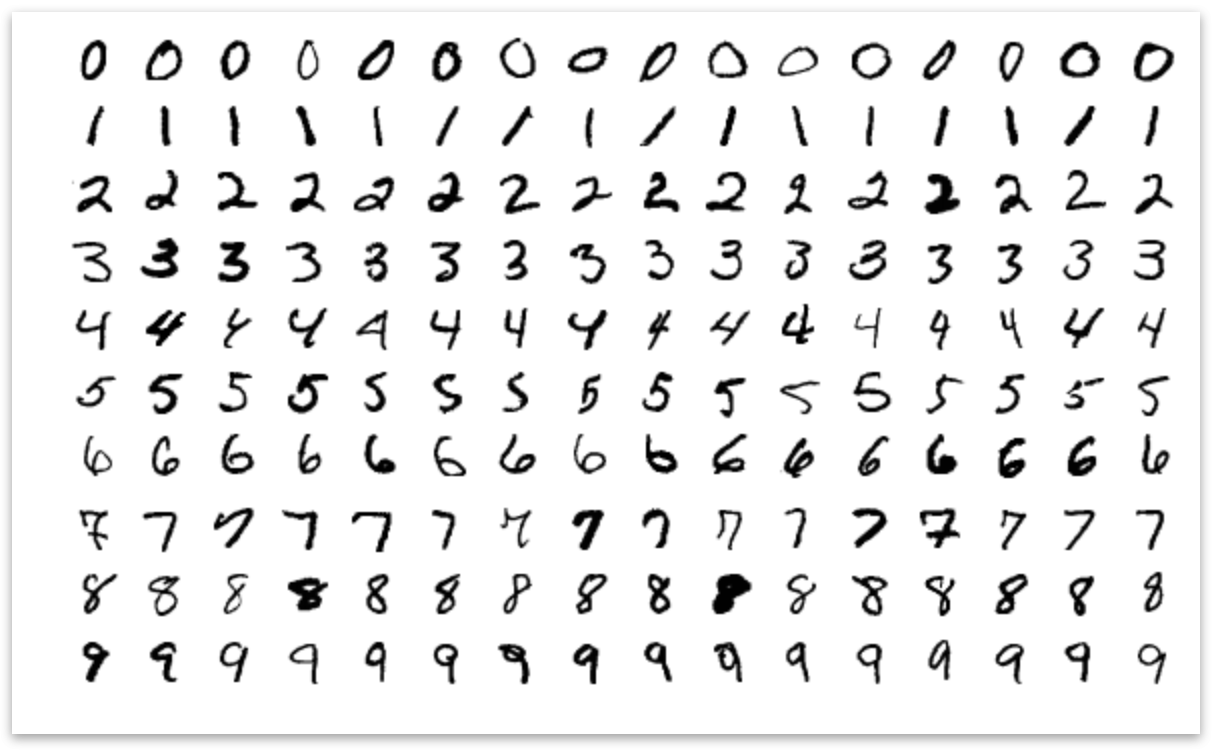
\includegraphics[width = 0.5 \textwidth]{media/ziffern.png}
\end{center}

Während wir problemlos die Ziffern oben erkennen können, ist das für einen Computer keinesfalls einfach, weil die gleiche Ziffer ganz unterschiedlich dargestellt werden kann. 
Für solche Probleme hat man grosse Erfolge durch den Einsatz von maschinellem Lernen erzielt. Dabei wird ein Programm zuerst trainiert, damit es die richtigen Muster erlernt.

Es gibt verschiedene Arten von lernenden Systemen. Für die Erkennung der Handschrift eignet sich ein sogenanntes neuronales Netz.
Etwas vereinfacht wird dabei ein grosser Vektor mit einer grossen Matrix multipliziert. Für     die Erkennung der Ziffern muss man sich das wie folgt vorstellen.
%Dabei wird das Programm zuerst «trainiert», damit der Computer die richtigen Muster «erlernt». Im Grunde geht das wie folgt:

\begin{center}
    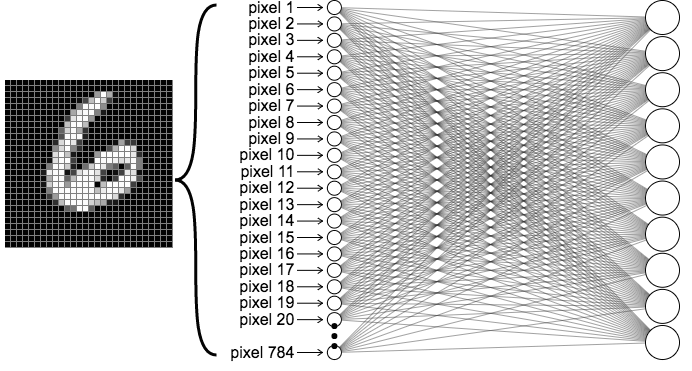
\includegraphics[width = 0.8 \textwidth]{media/mnist_1layer.png}
\end{center}

Das Programm erhält als Eingabe ein Bild. Im Beispiel ist das ein Graustufen-Bild mit $28\times28 =784$ Pixel. Nun soll der Computer entscheiden, um welche Zahl es sich dabei handelt.
Das Input-Bild kann als Vektor $\vec{v}$ mit 784 Komponenten gelesen werden, wobei z.B. in der 30. Komponente steht, wie dunkel der entsprechende Pixel (2. Pixel in der 2. Zeile) auf einer Skala von 0 bis 1 ist. Dieser Vektor wird dann mit einer $10\times784$-Matrix $M$ multipliziert und damit in einen Vektor $\vec{w} = M \cdot \vec{v}$ mit 10 Einträgen verwandelt. In diesem Vektor $\vec{w}$ steht dann, wie wahrscheinlich das Bild eine bestimmte Ziffer darstellt. So steht z.B. im 4. Eintrag von $\vec{w}$  die Wahrscheinlichkeit, dass es sich beim Bild um eine Vier handelt, im 10. Eintrag steht die Wahrscheinlichkeit für eine Null.
Die Frage ist nur noch: Wie lauten die 7840 Einträge der Matrix $M$? Die Kernidee des maschinellen Lernens ist, dass man den Computer diese Einträge selber lernen lässt! Dazu braucht es einiges an Mathematik. Mehr dazu im Schwerpunktfach AM oder im Ergänzungsfach I\dots


\clearpage
\section{Rechnen mit Matrizen}
\begin{LA}
    {}{}
    Mit Funktionen (oder Abbildungen) kann man rechnen!
    \begin{enumerate}
        \item \textbf{Zusammen:} Sei \( f(x) = x+2 \) und \( g(x) = x^2 \). Geben Sie die Gleichung der folgenden Funktionen an:

        \begin{enumerate}
            \item \( (f+g)(x) = \)
            \vspace{10pt}
            \item \( (f-g)(x) = \)
            \vspace{10pt}
            \item \( (3 \cdot f)(x) = \)
            \vspace{10pt}
            \item \( (f \circ g)(x) = \)
            \vspace{10pt}
            \item \( (g \circ f)(x) = \)
            \vspace{10pt}
        \end{enumerate}
        \item Analog für lineare Abbildungen! Gegeben sind die beiden Abbildungen:

        \[
        f \begin{pmatrix} x \\ y \end{pmatrix} = 
        \begin{pmatrix} 1 & 2 \\ 3 & 4 \end{pmatrix} 
        \begin{pmatrix} x \\ y \end{pmatrix}
        \quad \text{und} \quad
        g \begin{pmatrix} x \\ y \end{pmatrix} = 
        \begin{pmatrix} -2 & 4 \\ -3 & 1 \end{pmatrix} 
        \begin{pmatrix} x \\ y \end{pmatrix}
        \]
        
        Bestimmen Sie für die folgenden Funktionen die Bilder der Vektoren \( \vec{e}_1 = \begin{pmatrix} 1 \\ 0 \end{pmatrix} \) und \( \vec{e}_2 = \begin{pmatrix} 0 \\ 1 \end{pmatrix} \). Wie lautet dann die Matrix-Gleichung der Abbildung?
        \vspace{1cm}
        \begin{enumerate}
            \item \( (f+g)(\vec{e}_1) = \) \hfill \( (f+g)(\vec{e}_2) = \) \hfill Matrix von \( f+g \): \hfill
            \vspace{3cm}
            \item \( (f-g)(\vec{e}_1) = \) \hfill \( (f-g)(\vec{e}_2) = \) \hfill Matrix von \( f-g \):\hfill
            \vspace{3cm}
            
            \item \( (3 \cdot f)(\vec{e}_1) = \) \hfill \( (3 \cdot f)(\vec{e}_2) = \) \hfill Matrix von \( 3 \cdot f \):\hfill
            \vspace{3cm}
            \item \( (f \circ g)(\vec{e}_1) = \) \hfill \( (f \circ g)(\vec{e}_2) = \) \hfill Matrix von \( f \circ g \):\hfill
            \vspace{3cm}
            \item \( (g \circ f)(\vec{e}_1) = \) \hfill \( (g \circ f)(\vec{e}_2) = \) \hfill Matrix von \( g \circ f \):\hfill
            \vspace{3cm}
        \end{enumerate}
        
        \item Sei allgemein:

\[
f \begin{pmatrix} x \\ y \end{pmatrix} = 
\begin{pmatrix} a_{11} & a_{12} \\ a_{21} & a_{22} \end{pmatrix} 
\begin{pmatrix} x \\ y \end{pmatrix}
\quad \text{und} \quad
g \begin{pmatrix} x \\ y \end{pmatrix} = 
\begin{pmatrix} b_{11} & b_{12} \\ b_{21} & b_{22} \end{pmatrix} 
\begin{pmatrix} x \\ y \end{pmatrix}
\]

Leiten Sie die Matrix der Abbildung \( f \circ g \) her.
    \end{enumerate}
\end{LA}

\clearpage
Ähnlich wie mit Vektoren kann man auch mit Matrizen rechnen:
\begin{definition}
    {Addition und skalare Vielfache von Matrizen}{}
    Seien 
\[
A = \begin{pmatrix} a_{11} & a_{12} \\ a_{21} & a_{22} \end{pmatrix} 
\quad \text{und} \quad 
B = \begin{pmatrix} b_{11} & b_{12} \\ b_{21} & b_{22} \end{pmatrix}
\]
zwei Matrizen. Dann ist die Summe der beiden Matrizen definiert durch:

\[
A + B =
\begin{pmatrix} 
a_{11} + b_{11} & a_{12} + b_{12} \\ 
a_{21} + b_{21} & a_{22} + b_{22} 
\end{pmatrix}
\]

Sei \( \lambda \in \mathbb{R} \) eine reelle Zahl und 

\[
A = \begin{pmatrix} a_{11} & a_{12} \\ a_{21} & a_{22} \end{pmatrix}
\]

eine Matrix. Dann ist die Matrix \( \lambda \cdot A \) definiert durch:

\[
\lambda \cdot A =
\begin{pmatrix} 
\lambda \cdot a_{11} & \lambda \cdot a_{12} \\ 
\lambda \cdot a_{21} & \lambda \cdot a_{22} 
\end{pmatrix}
\]

Die Addition und die skalaren Vielfachen von \( 3 \times 3 \)-Matrizen werden analog definiert.

\end{definition}

\begin{bsp}
    {}{}
    \[
\begin{pmatrix} 1 & 2 \\ 3 & 4 \end{pmatrix} 
+ 
\begin{pmatrix} -2 & 4 \\ -3 & 1 \end{pmatrix} 
=
\begin{pmatrix} -1 & 6 \\ 0 & 5 \end{pmatrix}
\]

\[
3 \cdot 
\begin{pmatrix} 1 & 2 \\ 3 & -4 \end{pmatrix} 
=
\begin{pmatrix} 3 & 6 \\ 9 & -12 \end{pmatrix}
\]

\end{bsp}

Für diese Operationen gelten die üblichen Rechengesetze:
\begin{multicols}{2}
    \begin{itemize}
        %\item \( 1 \cdot A = A \)
        %\item \( 0 \cdot A = O \)
        \item \( \lambda \cdot A = A \cdot \lambda \)
        \item \( \lambda \cdot (\mu \cdot A) = (\lambda \cdot \mu) \cdot A \)
        \item \( (\lambda + \mu) \cdot A = \lambda \cdot A + \mu \cdot A \)
        \item \( \lambda \cdot (A + B) = \lambda \cdot A + \lambda \cdot B \)
        \item \( A + (B + C) = (A + B) + C \)
        \item \( (A + B) \cdot \vec{v} = A \cdot \vec{v} + B \cdot \vec{v} \)
        \item \( (\lambda \cdot A) \cdot \vec{v} = \lambda \cdot (A \cdot \vec{v}) \)
    \end{itemize}
    \end{multicols}
    
    % \textbf{Fazit:} Man kann mit Matrizen rechnen wie mit Zahlen!
\begin{bsp}
    {Matrixgleichung}{}
    Für welche Matrix \( X \) gilt

    \[
    2 \cdot 
    \begin{pmatrix} 1 & 2 \\ 1 & 1 \end{pmatrix} 
    + 3 \cdot X 
    - \begin{pmatrix} 0 & 2 \\ 2 & 1 \end{pmatrix} 
    = X \quad ?
    \]

    So eine Gleichung kann man lösen, als würde man mit Zahlen operieren. Durch Isolieren von \( X \) erhält man:

    \[
    2X = \begin{pmatrix} 0 & 2 \\ 2 & 1 \end{pmatrix} 
    - 2 \cdot \begin{pmatrix} 1 & 2 \\ 1 & 1 \end{pmatrix} = \begin{pmatrix} -2 & -2 \\ 0 & -1 \end{pmatrix}
    \]

    % \[
    % = \begin{pmatrix} 0 - 2 & 2 - 4 \\ 2 - 2 & 1 - 2 \end{pmatrix}
    % = \begin{pmatrix} -2 & -2 \\ 0 & -1 \end{pmatrix}
    % \]

    \[
    X = \frac{1}{2} \cdot \begin{pmatrix} -2 & -2 \\ 0 & -1 \end{pmatrix}
    = \begin{pmatrix} -1 & -1 \\ 0 & -\frac{1}{2} \end{pmatrix}
    \]
\end{bsp}

Das Produkt von zwei Matrizen wird wie folgt definiert:
\begin{definition}
    {Produkt von 2x2 Matrizen}{}
    Seien 
    \[
    A = \begin{pmatrix} a_{11} & a_{12} \\ a_{21} & a_{22} \end{pmatrix}
    \quad \text{und} \quad
    B = \begin{pmatrix} b_{11} & b_{12} \\ b_{21} & b_{22} \end{pmatrix}
    \]
    zwei Matrizen. Dann ist das Produkt der beiden Matrizen definiert durch:

    \[
    A \cdot B =
    \begin{pmatrix} 
    a_{11} b_{11} + a_{12} b_{21} & a_{11} b_{12} + a_{12} b_{22} \\ 
    a_{21} b_{11} + a_{22} b_{21} & a_{21} b_{12} + a_{22} b_{22}
    \end{pmatrix}
    \]

\end{definition}

\begin{bsp}
    {Berechnung eines Matrixprodukts}{}
    \vspace*{1cm}
    \(
\begin{pmatrix} 1 & 2 \\ 3 & 4 \end{pmatrix} 
\cdot 
\begin{pmatrix} -2 & 4 \\ -3 & 1 \end{pmatrix} = 
\)
\vspace*{1cm}
\end{bsp}

Analog werden auch grössere Matrizen Multipliziert:

\begin{bsp}
    {Produkt von 3x3-Matrizen}{}
    \vspace*{1cm}
    $
    \begin{pmatrix} 1 & 0 & -1 \\ 2 & 3 & 0 \\ -2 & 2 & 1 \end{pmatrix} 
    \cdot 
    \begin{pmatrix} 1 & 2 & 3 \\ 4 & 5 & 6 \\ 7 & 8 & 9 \end{pmatrix} =
    $
    \vspace*{1cm}
\end{bsp}

Vielleicht fragen Sie sich an dieser Stelle, wieso das Produkt von zwei Matrizen so kompliziert definiert ist. Es wäre doch viel simpler, wenn man einfach die einzelnen Einträge miteinander multiplizieren würde!  

Der Grund liegt darin, dass das so definierte Produkt eine wichtige Eigenschaft erfüllt. Es gilt nämlich für alle Matrizen \( A \) und \( B \) und alle Vektoren \( \vec{v} \), dass:

\[
A \cdot (B \cdot \vec{v}) = (A \cdot B) \cdot \vec{v}
\]

Die Bedeutung dieser Eigenschaft der Matrix-Multiplikation erschliesst sich, wenn man Matrizen als lineare Abbildungen auffasst.  

Zur Erinnerung:

\begin{definition}
    {Komposition / Verkettung von Abbildungen}{}
    Seien \( f \) und \( g \) zwei Abbildungen. Dann ist die Komposition (oder Verkettung) \( f \circ g \) von \( f \) und \( g \) die Abbildung, definiert durch:

    \[
    (f \circ g)(\vec{v}) = f(g(\vec{v}))
    \]


\end{definition}
Wenn beispielsweise \( f \) eine Drehung ist und \( g \) eine Spiegelung, dann ist \( f \circ g \) die Abbildung, bei welcher die Punkte zuerst gespiegelt und anschliessend gedreht werden.  
(Achten Sie auf die Reihenfolge: Bei \( f \circ g \) wird zuerst \( g \) ausgeführt, anschliessend \( f \).)

Nun lässt sich die obengenannte Eigenschaft $A \cdot (B \cdot \vec{v}) = (A \cdot B) \cdot \vec{v}$ so verstehen:

\begin{satz}
    {Komposition und Matrixmultiplikation}{}
    Seien \( f \) und \( g \) zwei lineare Abbildungen. Weiter sei \( A \) die Matrix von \( f \) und \( B \) jene von \( g \).  

    Dann ist \( f \circ g \) auch eine lineare Abbildung, und die dazugehörige Matrix ist:
    $
    A \cdot B
    $

\end{satz}
\begin{bsp}
    {}{}
    Sei 
    \[
    A = \begin{pmatrix} 1 & -2 \\ 3 & 4 \end{pmatrix}
    \]
    die Matrix der linearen Abbildung \( f \) und 
    \[
    B = \begin{pmatrix} 5 & -6 \\ 7 & 8 \end{pmatrix}
    \]
    jene der Abbildung \( g \).  

    Dann hat die Abbildung \( f \circ g \) die Matrix:
    \begin{align*}
    A \cdot B &=
    \begin{pmatrix} 1 & -2 \\ 3 & 4 \end{pmatrix}
    \cdot
    \begin{pmatrix} 5 & -6 \\ 7 & 8 \end{pmatrix}
    \\
    &=
    \begin{pmatrix} 
    1 \cdot 5 + (-2) \cdot 7 & 1 \cdot (-6) + (-2) \cdot 8 \\ 
    3 \cdot 5 + 4 \cdot 7 & 3 \cdot (-6) + 4 \cdot 8 
    \end{pmatrix}\\
    &=
    \begin{pmatrix} 
    -9 & -22 \\ 43 & 14 
    \end{pmatrix}
\end{align*}

\end{bsp}

\clearpage
\begin{ueb}
    {}{}
    \begin{enumerate}
        \item Sei \( f: \mathbb{R}^2 \to \mathbb{R}^2 \) die Spiegelung an der Geraden \( y = x \) und \( g: \mathbb{R}^2 \to \mathbb{R}^2 \) die Drehung um den Ursprung um \( 90^\circ \) gegen den Uhrzeigersinn.
        \begin{enumerate}
            \item Bestimmen Sie die Matrix \( A \) von \( f \) und die Matrix \( B \) von \( g \).
            \item Bestimmen Sie die Matrix \( C \) der Verkettung \( g \circ f \).
            \item \( C \) ist die Matrix einer Spiegelung. An welcher Achse wird gespiegelt?
            \item Bestimmen Sie die Matrix \( D \) der Verkettung \( f \circ g \) (andere Reihenfolge).
            \item Auch \( D \) ist die Matrix einer Spiegelung. Was ist diesmal die Achse?
        \end{enumerate}
    
        \item In Aufgabe 1. wurde deutlich, dass die Matrixmultiplikation im Gegensatz zum Produkt von Zahlen nicht kommutativ ist (das heisst: im Allgemeinen gilt \( A \cdot B \neq B \cdot A \)).
        Ein weiterer Unterschied zur Multiplikation von Zahlen zeigt sich in diesen Übungen:
        \begin{enumerate}
            \item Berechnen Sie  
            \[
            \begin{pmatrix} 1 & 2 \\ 2 & 4 \end{pmatrix} 
            \cdot 
            \begin{pmatrix} -2 & 6 \\ 1 & -3 \end{pmatrix}
            \]
            \item Berechnen Sie  
            \[
            \begin{pmatrix} 0 & 0 \\ 1 & 0 \end{pmatrix}^2 
            =
            \begin{pmatrix} 0 & 0 \\ 1 & 0 \end{pmatrix} 
            \cdot 
            \begin{pmatrix} 0 & 0 \\ 1 & 0 \end{pmatrix}
            \]
        \end{enumerate}
    
        \item Sei \( f: \mathbb{R}^3 \to \mathbb{R}^3 \) die Spiegelung an der $yz$-Ebene. 
        \begin{enumerate}
            \item Bestimmen Sie die Matrix \( M \) von \( f \) und berechnen Sie anschliessend \( M^2 \).
            \item Interpretieren Sie das Resultat.
        \end{enumerate}
    
        \item Sei \( A \) die \( 2 \times 2 \)-Matrix der Drehung um den Winkel \( \varphi \) um den Ursprung und \( B \) jene der Drehung um den Winkel \( \psi \) um den Ursprung.
        \begin{enumerate}
            \item Geben Sie die Matrizen \( A \) und \( B \) an.
            \item Berechnen Sie anschliessend \( A \cdot B \).
        \end{enumerate}
    \end{enumerate}
    
\end{ueb}

\begin{ueb}
    {Programmieraufgabe}{}
    Ergänzen Sie die Klasse \lstinline|matrix2x2| um die Methoden
    \begin{itemize}
        \item \lstinline|plus(self, b)| für die Addition zweier Matrizen.
        \item \lstinline|minus(self, b)| für die Subtraktion zweier Matrizen. 
        \item \lstinline|mal_skalar(self, x)| für die Multiplikation mit einem Skalar (eine Zahl $x$).
        \item \lstinline|mal_mat(self, b)| für die Multiplikation zweier Matrizen.
    \end{itemize}
\end{ueb}

\begin{ueb}
    {Weiterführenden Programmieraufgabe: Unterklassen}{}
    Wie kann man Drehmatrizen als einen Spezialfall von Matrizen in Python realisieren? Nun das geht mit einer sogenannten Unterklasse. Der Code dazu lautet wie folgt:
    \begin{lstlisting}
class drehmatrix2x2(matrix2x2):
    def __init__(self, winkel):
        a = math.cos(winkel)
        b = math.sin(winkel)
        super().__init__(a, -b, b, a))
        self.winkel = winkel \end{lstlisting}

 Die Erklärung dazu:
\begin{itemize}
    \item In Zeile 1 wird die Klasse mit dem Namen \lstinline|drehmatrix2x2| definiert. Der Verweis auf \lstinline|matrix2x2| in der Klammer legt fest, dass es sich dabei um eine Unterklasse von \lstinline|matrix2x2| handelt.
    \item In Zeile 2 wird der Konstruktor definiert.
    \item Zeilen 3 und 4 definieren zwei Hilfsvariablen, um die Einträge der Matrix zu bestimmen. Für die Verwendung der Funktionen \lstinline|math.sin(winkel)| und \lstinline|math.cos(winkel)|, muss davor die Bibliothek \lstinline|import math| importiert werden.
    \item Mit \lstinline|super()| wird auf die Methoden der Oberklasse zugegriffen. In Zeile 5 wird also der Konstruktor der Klasse \lstinline|matrix2x2| aufgerufen, damit ein Matrix-Objekt gebildet wird.
    \item In Zeile 6 wird ein zusätzlich Attribut für Drehmatrizen definiert. Mit \lstinline|d.winkel| kann fortan auf den Drehwinkel zugegriffen werden.
\end{itemize}

\begin{enumerate}
    \item Kopieren Sie den Code und versuchen Sie, eine Drehmatrix mit einer anderen Matrix zu multiplizieren.
    \item Die Matrix einer Spiegelung \( S_g \) an einer Ursprungsgeraden mit dem Winkel \( \alpha \) zur positiven $x$-Achse ist:
    \[
    S_g =
    \begin{pmatrix} 
    \cos 2\alpha & \sin 2\alpha \\ 
    \sin 2\alpha & -\cos 2\alpha 
    \end{pmatrix}
    \]

    Definieren Sie eine neue Unterklasse \lstinline|spiegelmatrix2x2(matrix2x2)|.
    
\end{enumerate} 


\end{ueb}






\clearpage
\emph{Lösungen:}
\begin{enumerate}
    \item \textbf{Spiegelung und Drehung}
    \begin{enumerate}
        \item \( A = \begin{pmatrix} 0 & 1 \\ 1 & 0 \end{pmatrix} \), \quad \( B = \begin{pmatrix} 0 & -1 \\ 1 & 0 \end{pmatrix} \)
        \item \( C = B \cdot A = \begin{pmatrix} -1 & 0 \\ 0 & 1 \end{pmatrix} \)
        \item An der $y$-Achse
        \item \( D = \begin{pmatrix} 1 & 0 \\ 0 & -1 \end{pmatrix} \)
        \item An der $x$-Achse
    \end{enumerate}

    \item \textbf{Produkte}
    \begin{enumerate}
        \item \[
        \begin{pmatrix} 1 & 2 \\ 2 & 4 \end{pmatrix} 
        \cdot 
        \begin{pmatrix} -2 & 6 \\ 1 & -3 \end{pmatrix} 
        =
        \begin{pmatrix} 0 & 0 \\ 0 & 0 \end{pmatrix}
        \]
        Obwohl das Produkt die Nullmatrix ergibt, ist keiner der beiden Faktoren die Nullmatrix!
        \item \[
        \begin{pmatrix} 0 & 0 \\ 1 & 0 \end{pmatrix}^2 
        =
        \begin{pmatrix} 0 & 0 \\ 0 & 0 \end{pmatrix}
        \]
    \end{enumerate}

    \item \textbf{Matrix der Spiegelung in \( \mathbb{R}^3 \)}
    \begin{enumerate}
        \item \[
        M = \begin{pmatrix} -1 & 0 & 0 \\ 0 & 1 & 0 \\ 0 & 0 & 1 \end{pmatrix}, 
        \quad M^2 = \begin{pmatrix} 1 & 0 & 0 \\ 0 & 1 & 0 \\ 0 & 0 & 1 \end{pmatrix}
        \]
        Das ist die Matrix der Identität \( \text{id}(\vec{v}) = \vec{v} \). Das muss so sein, weil jeder Punkt nach zweimaligem Spiegeln auf sich selbst abgebildet wird.
    \end{enumerate}

    \item \textbf{Drehungsmatrizen}
    \begin{enumerate}
        \item \[
        A = \begin{pmatrix} \cos(\varphi) & -\sin(\varphi) \\ \sin(\varphi) & \cos(\varphi) \end{pmatrix}, 
        \quad B = \begin{pmatrix} \cos(\psi) & -\sin(\psi) \\ \sin(\psi) & \cos(\psi) \end{pmatrix}
        \]

        \item Berechnung von \( A \cdot B \):

        \[
        A \cdot B =
        \begin{pmatrix} 
        \cos(\varphi) \cos(\psi) - \sin(\varphi) \sin(\psi) & -(\sin(\varphi) \cos(\psi) + \cos(\varphi) \sin(\psi)) \\ 
        \sin(\varphi) \cos(\psi) + \cos(\varphi) \sin(\psi) & \cos(\varphi) \cos(\psi) - \sin(\varphi) \sin(\psi) 
        \end{pmatrix}
        \]

        \[
        =
        \begin{pmatrix} \cos(\varphi + \psi) & -\sin(\varphi + \psi) \\ \sin(\varphi + \psi) & \cos(\varphi + \psi) \end{pmatrix}
        \]

        Das Resultat ist die Matrix einer Drehung um den Winkel \( \varphi + \psi \).  
        Wobei für den letzten Schritt die Additionstheoreme verwendet wurden:

        \[
        \sin(\alpha + \beta) = \sin(\alpha) \cos(\beta) + \cos(\alpha) \sin(\beta)
        \]
        
        \[
        \cos(\alpha + \beta) = \cos(\alpha) \cos(\beta) - \sin(\alpha) \sin(\beta)
        \]
    \end{enumerate}
\end{enumerate}

\clearpage
\section{Inverse Abbildungen und inverse Matrizen}
\subsection{Begriffe und Formeln}
\begin{LA}
{Invertierbare Abbildung}{Inverse}
Sei 
\[
A = \begin{pmatrix} 3 & 16 \\ 1 & 4 \end{pmatrix}
\]
die Matrix einer linearen Abbildung \( f \) und 
\[
B = \begin{pmatrix} -1 & 4 \\ \frac{1}{4} & -\frac{3}{4} \end{pmatrix}
\]
jene von \( g \). Weiter sei 
\[
\vec{v} = \begin{pmatrix} x \\ y \end{pmatrix}
\]
ein beliebiger Vektor.

\begin{enumerate}
    \item Berechnen Sie \( \vec{w} = f(\vec{v}) \).
    \item Berechnen Sie nun \( g(\vec{w}) \).
    \item Berechnen Sie das Matrix-Produkt \( B \cdot A \).
\end{enumerate}
\end{LA}
\clearpage
\begin{LA}{nicht invertierbare Abbildung}{keineInverse}
Offenbar macht in \Cref{LA:Inverse} die Matrix $B$ die Wirkung von $A$ rückgängig. Betrachten Sie nun die Matrix
$$C = \begin{pmatrix}
    1&2 \\3&6
\end{pmatrix} $$

\begin{enumerate}
    \item Berechnen Sie $C\cdot\begin{pmatrix}
        2\\0
    \end{pmatrix}$ und $C\cdot\begin{pmatrix}
        0\\1
    \end{pmatrix}$.
    \item Berechnen Sie allgemein $C\cdot\begin{pmatrix}
        x\\y
    \end{pmatrix}$ und begründen Sie, wieso es keinen Vektor $\vec{v}$ gibt, mit der Eigenschaft, dass $C\cdot\vec{v} = \begin{pmatrix}
        1 \\2
    \end{pmatrix}$ ist.
    \item Geben Sie zwei Gründe an, wieso es keine Matrix gibt, welche die Wirkung von $C$ rückgängig macht.
\end{enumerate}
\end{LA}


















\clearpage
In der \Cref{LA:Inverse} haben Sie zwei zueinander inverse Abbildungen betrachtet. In diesem Kapitel wird genau definiert, was man unter einer inversen Abbildung versteht, und wir werden eine Formel angeben, mit der man die Inverse einer linearen Abbildung bestimmen kann.

\begin{definition}
    {Identität und Einheitsmatrix}{}
    Die lineare Abbildung mit der Eigenschaft, dass jeder Vektor auf sich selbst abgebildet wird, nennt man die \textbf{Identitätsabbildung}.  

\textbf{Notation:} \( \text{id} \), also  
\[
\text{id}(\vec{v}) = \vec{v} \quad \text{für alle Vektoren } \vec{v}.
\]

Die Abbildungsmatrix der Identitätsabbildung heisst \textbf{Einheitsmatrix}.  

In \( \mathbb{R}^2 \) gilt:
\[
E = \begin{pmatrix} 1 & 0 \\ 0 & 1 \end{pmatrix}.
\]
% In \( \mathbb{R}^3 \) gilt:

% \[
% E = \begin{pmatrix} 1 & 0 & 0 \\ 0 & 1 & 0 \\ 0 & 0 & 1 \end{pmatrix}.
% \]
\end{definition}
Die Identitätsabbildung ist das \textbf{neutrale Element} bezüglich der Komposition von Abbildungen. Für jede Abbildung \( f \) gilt:
\[
f \circ \text{id} = \text{id} \circ f = f
\]
Analog ist die Matrix \( E \) das \textbf{neutrale Element} bezüglich der Matrixmultiplikation. Für jede andere Matrix \( A \) gilt:
\[
A \cdot E = E \cdot A = A
\]

\begin{definition}
    {Inverse Abbildung und inverse Matrix}{}
    Seien \( f \) und \( f^{-1} \) zwei lineare Abbildungen mit der Eigenschaft:
    \[
    f \circ f^{-1} = \text{id}
    \]
    Dann nennt man \( f^{-1} \) die \textbf{inverse Abbildung} zu \( f \).

    \textbf{Analog:}  

    Seien \( A \) und \( A^{-1} \) zwei Matrizen mit der Eigenschaft, dass
    \[
    A \cdot A^{-1} = E.
    \]
    Dann nennt man \( A^{-1} \) die \textbf{inverse Matrix} zu \( A \).
\end{definition}

\begin{bsp}
    {}{}
    Die folgenden Matrizen sind invers zueinander:
    \[
    A = \begin{pmatrix} 3 & 16 \\ 1 & 4 \end{pmatrix}, \quad
    B = \begin{pmatrix} -1 & 4 \\ \frac{1}{4} & -\frac{3}{4} \end{pmatrix}
    \]
    Es gilt nämlich:
    \[
    A \cdot B =
    \begin{pmatrix} 
    3 \cdot (-1) + 16 \cdot \frac{1}{4} & 3 \cdot 4 + 16 \cdot \left(-\frac{3}{4} \right) \\ 
    1 \cdot (-1) + 4 \cdot \frac{1}{4} & 1 \cdot 4 + 4 \cdot \left(-\frac{3}{4} \right)
    \end{pmatrix}
     =
    \begin{pmatrix} 
    -3 + 4 & 12 - 12 \\ 
    -1 + 1 & 4 - 3
    \end{pmatrix}
    =
    \begin{pmatrix} 1 & 0 \\ 0 & 1 \end{pmatrix}
    \]

\end{bsp}
\clearpage
% \begin{bsp}
%     {}{}
%     Gegeben ist die Matrix:

% \[
% A =
% \begin{pmatrix} a_{11} & a_{12} \\ a_{21} & a_{22} \end{pmatrix}.
% \]

% Zeigen Sie, dass die Matrix:

% \[
% B = \frac{1}{a_{11} a_{22} - a_{12} a_{21}}
% \begin{pmatrix} a_{22} & -a_{12} \\ -a_{21} & a_{11} \end{pmatrix}
% \]

% die Inverse von \( A \) ist.

% \vspace*{10cm}

% \end{bsp}

\begin{bsp}
    {Formel für die Inverse}{}
        Gegeben ist die Matrix:
\[
A =
\begin{pmatrix} a & b \\ c & d \end{pmatrix}.
\]
Gesucht ist deren inverse Matrix 
\[
A^{-1} =
\begin{pmatrix} w & x \\ y & z \end{pmatrix}.
\]

\vspace*{18cm}
\end{bsp}
\clearpage



\begin{definition}
    {Determinante}{}
    Sei $$A= \begin{pmatrix}
        a & b \\ c & d
    \end{pmatrix}$$
    Die Zahl 
    $$ \det(A) = ad-bc$$
    nennt man die \emph{Determinante} der Matrix $A$.
\end{definition}

\begin{satz}
    {Berechnung der inversen Matrix}{}
    Sei \( A \) die Matrix:
    $$A= \begin{pmatrix}
        a & b \\ c & d
    \end{pmatrix}$$
    mit Determinante:
    $$ \det(A) = ad-bc$$
    Falls \( \det(A) \neq 0 \) gilt:
    \[
    A^{-1} = \phantom{\frac{1}{\det(A)}
    \begin{pmatrix} a_{22} & -a_{12} \\ -a_{21} & a_{11} \end{pmatrix}}
    \]

    Falls \( \det(A) = 0 \) hat die Matrix \( A \) keine Inverse.

\end{satz}
\begin{bsp}
    {}{}
    Die Matrix 
\[
A =
\begin{pmatrix} 1 & 2 \\ 3 & 4 \end{pmatrix}
\]
ist invertierbar, denn 

\[
\det(A) = 1 \cdot 4 - 2 \cdot 3 = -2.
\]

Es gilt:

\[
A^{-1} = \frac{1}{-2} 
\begin{pmatrix} 4 & -2 \\ -3 & 1 \end{pmatrix}
=
\begin{pmatrix} -2 & 1 \\ \frac{3}{2} & -\frac{1}{2} \end{pmatrix}
\]

\end{bsp}

\begin{bsp}
    {Nicht-invertierbare Matrix}{}
    Die Matrix $B=\begin{pmatrix}
        1&2 \\3&6
    \end{pmatrix}$ ist nicht invertierbar, denn
    $$\det B = 1\cdot 6 - 3\cdot 2 = 0$$
    Die entsprechende lineare Abbildung ist auch nicht invertierbar, denn
    $$ B\begin{pmatrix}
        2 \\0 
    \end{pmatrix}  = \begin{pmatrix}
        2 \\6
    \end{pmatrix} \qquad \text{und} \qquad B\begin{pmatrix}
        0 \\1 
    \end{pmatrix} = \begin{pmatrix}
        2 \\6
    \end{pmatrix},$$
    womit die Abbildung nicht injektiv ist (surjektiv ist sie auch nicht, siehe \Cref{LA:keineInverse}). 
\end{bsp}
\pagebreak
\begin{ueb}
    {}{}
    \begin{enumerate}
        
    \item Gegeben ist die Matrix der linearen Abbildung \( f \):

    \[
    A = \begin{pmatrix}
    3 & 2 \\
    5 & 4
    \end{pmatrix}
    \]
    
    \begin{enumerate}
      \item Bestimmen Sie die Matrix der inversen Abbildung \( f^{-1} \).
      \item Bestimmen Sie das Urbild des Vektors 
      \[
      \vec{v} = \begin{pmatrix}
      -10 \\
      8
      \end{pmatrix},
      \]
      d.\,h. denjenigen Vektor, der durch \( f \) auf \( \vec{v} \) abgebildet wird.
    \end{enumerate}

    \item Die Abbildung \( f \) ist die Spiegelung an der Geraden \( y = x \),  
    die Abbildung \( g \) ist die Drehung um den Ursprung \( O \) um \( 30^\circ \) gegen den Uhrzeigersinn.
    
    \begin{enumerate}
      \item Ermitteln Sie die Matrix \( A_f \) der Abbildung \( f \). Welche geometrische Bedeutung hat diese Matrix?
      \item Ermitteln Sie die Matrix \( A_g \) der Abbildung \( g \). Welche geometrische Bedeutung hat diese Matrix?
      \item Berechnen Sie \( A_f^{-1} \) und \( A_g^{-1} \).
      \item Zeigen Sie, dass $(A_f \cdot A_g)^{-1} = A_g^{-1} \cdot A_f^{-1}$ gilt. Geben Sie eine geometrische Deutung an.
      \item Bestimmen Sie die Matrix \( A_h \) einer Abbildung \( h \), sodass gilt:
      \[
      h \circ f = g
      \]
      \item Bestimmen Sie die Matrix \( A_h \) einer Abbildung \( h \), sodass gilt:
      \[
      f \circ h = g
      \]
    %   \textit{Hinweis: Multiplizieren Sie die Gleichung von links mit der Inversen von \( A_f \), also \( A_f^{-1} \).}
    \end{enumerate}
    \item Die Matrix einer Drehung gegen den Uhrzeigersin um den Ursprung um den Winkel \( \alpha \) ist gegeben durch:
    \[
    A_\alpha = \begin{pmatrix}
    \cos(\alpha) & -\sin(\alpha) \\
    \sin(\alpha) & \cos(\alpha)
    \end{pmatrix}
    \]
    Überlegen Sie sich, wie die Matrix der Inversen Abbildung aussieht. Berechnen Sie die Inverse der Matrix \( A_\alpha \) und überprüfen Sie Ihre Überlegung.
    \end{enumerate}
\end{ueb}

\begin{ueb}
    {Programmieraufgabe}{}
    Ergänzen Sie die Klasse \lstinline|matrix2x2| um die Methoden
    \begin{itemize}
        \item \lstinline|det(self)| für die Berechnung der Determinante einer Matrix.
        \item \lstinline|inv(self)| für die Berechnung der Inversen einer Matrix.
    \end{itemize}
\end{ueb}


\clearpage
\emph{Lösungen}
\begin{enumerate}

    \item
    \begin{enumerate}
      \item \( A^{-1} = \begin{pmatrix} 2 & -1 \\ -5/2 & 3/2 \end{pmatrix} \)
      \item \( \vec{u} = \begin{pmatrix} -28\\ 37 \end{pmatrix} \)
    \end{enumerate}
  
    \item
    \begin{enumerate}
      \item \( A_f = \begin{pmatrix} 0 & 1 \\ 1 & 0 \end{pmatrix} \)
      \item \( A_g = \begin{pmatrix} \cos(30^\circ) & -\sin(30^\circ) \\ \sin(30^\circ) & \cos(30^\circ) \end{pmatrix}
              = \begin{pmatrix} \frac{\sqrt{3}}{2} & -\frac{1}{2} \\ \frac{1}{2} & \frac{\sqrt{3}}{2} \end{pmatrix} \)
      \item \( A_f^{-1} = A_f = \begin{pmatrix} 0 & 1 \\ 1 & 0 \end{pmatrix} \),
            \quad
            \( A_g^{-1} = \begin{pmatrix} \frac{\sqrt{3}}{2} & \frac{1}{2} \\ -\frac{1}{2} & \frac{\sqrt{3}}{2} \end{pmatrix} \)
      \item \dots
        \item \( A_h = A_g \cdot A_f^{-1} = \begin{pmatrix} -\frac{1}{2} & \frac{\sqrt{3}}{2} \\ \frac{\sqrt{3}}{2} & \frac{1}{2} \end{pmatrix} \)
      \item \( A_h = A_f^{-1} \cdot A_g =  \begin{pmatrix} \frac{1}{2} & \frac{\sqrt{3}}{2} \\ \frac{\sqrt{3}}{2} & -\frac{1}{2} \end{pmatrix} \)
    \end{enumerate}
    \item $$ A^{-1} = \begin{pmatrix}
        \cos(-\alpha) & -\sin(-\alpha) \\
        \sin(-\alpha) & \cos(-\alpha)
    \end{pmatrix} = \begin{pmatrix}
        \cos(\alpha) & \sin(\alpha) \\
        -\sin(\alpha) & \cos(\alpha)
    \end{pmatrix}$$
  
  \end{enumerate}

  \clearpage






























  \subsection{Geometrische Bedeutung der Determinante}
  \begin{LA}
      {Geometrische Bedeutung der Determinante}{determinanteUndFläche}
      In dieser Aufgabe geht es um die geometrische Bedeutung der Determinante einer Matrix.

      Betrachten Sie dazu eine lineare Abbildung \( f \) mit der Abbildungsmatrix
      \[
      A = \begin{pmatrix}
      a_{11} & a_{12}  \\
      a_{21} & a_{22}
      \end{pmatrix}.
      \]
      
      Die Basisvektoren
      \[
      \vec{e}_1 = \begin{pmatrix} 1 \\ 0 \end{pmatrix}, \quad
      \vec{e}_2 = \begin{pmatrix} 0 \\ 1 \end{pmatrix}
      \]
      spannen ein Quadrat mit dem Flächeninhalt \( I = 1 \) auf.

      Unter der Abbildung $f$ wird das Quadrat in ein Viereck abgebildet. Im Folgenden soll der Flächeninhalt $I'$ dieses Vierecks berechnet werden. 
      
      \begin{enumerate}
        \item Wieso ist das Bild des Einheitsquadrates unter der Abbildung $f$ ein Parallelogramm, dessen Ecken die folgenden Koordinaten haben?
        \begin{center}
            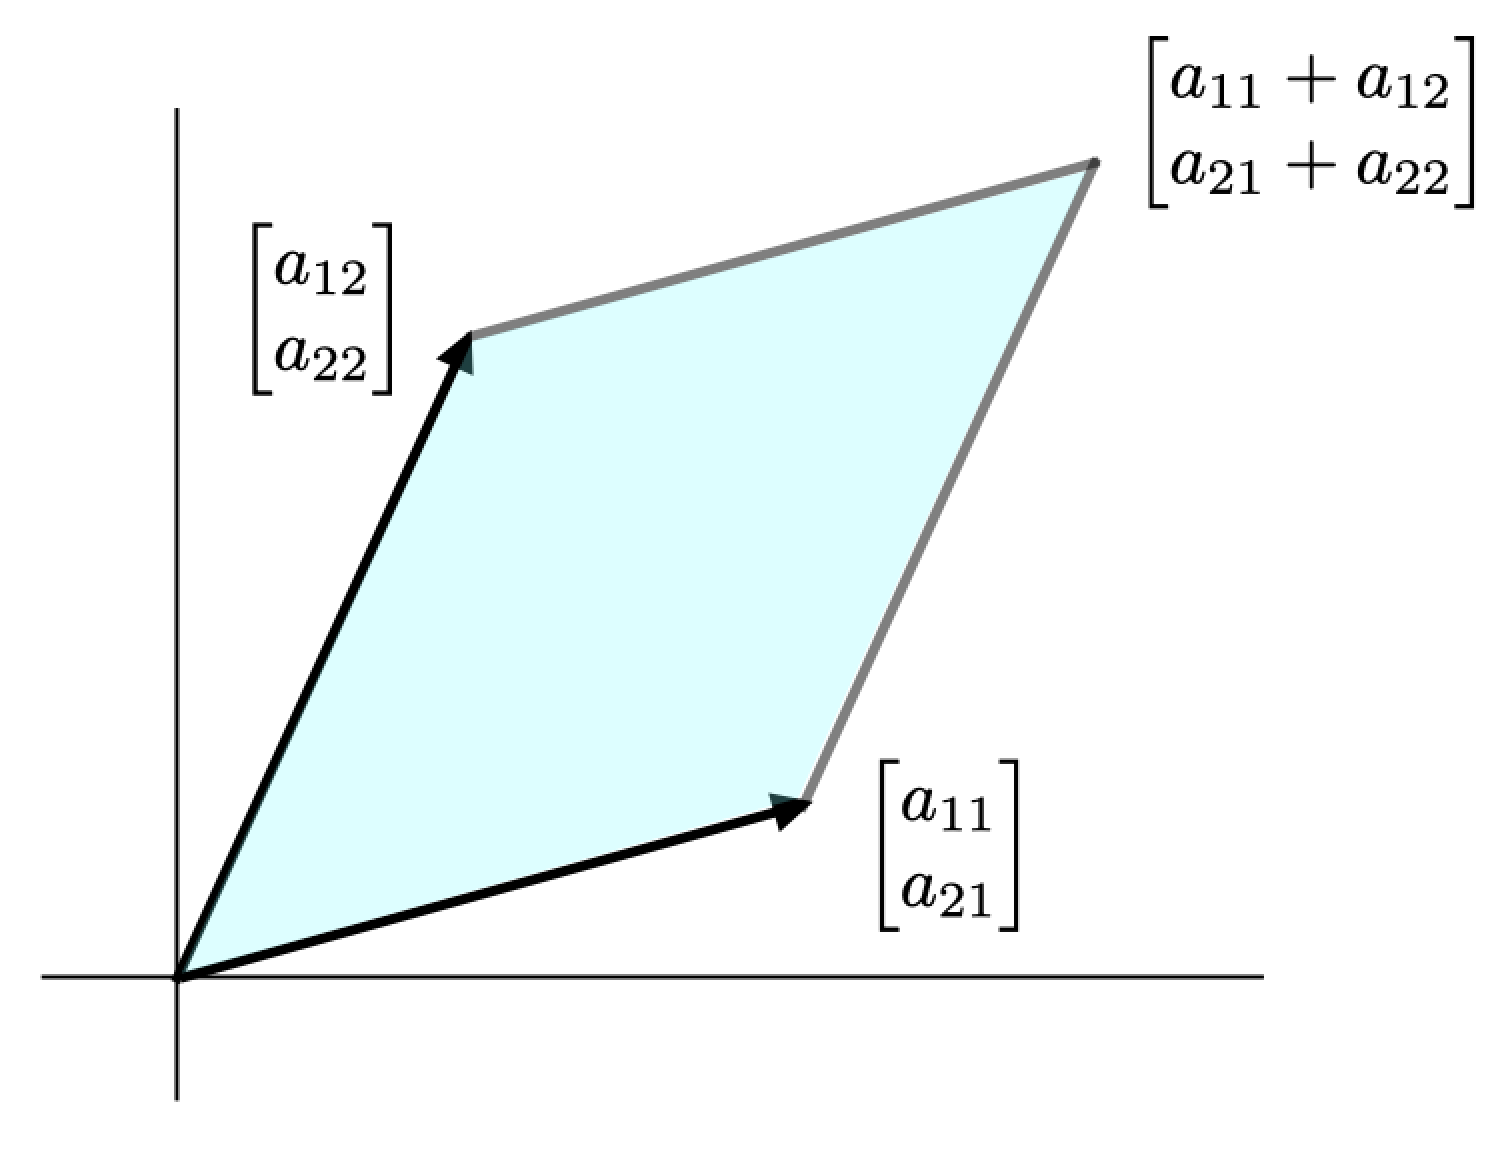
\includegraphics[width = 0.4\textwidth]{media/determinateFlaeche1.png}
        \end{center}
        \item Welchen Flächeninhalt \( I' \) hat das Parallelogramm? Nutzen Sie die folgende Hilfsfigur:
        \begin{center}
            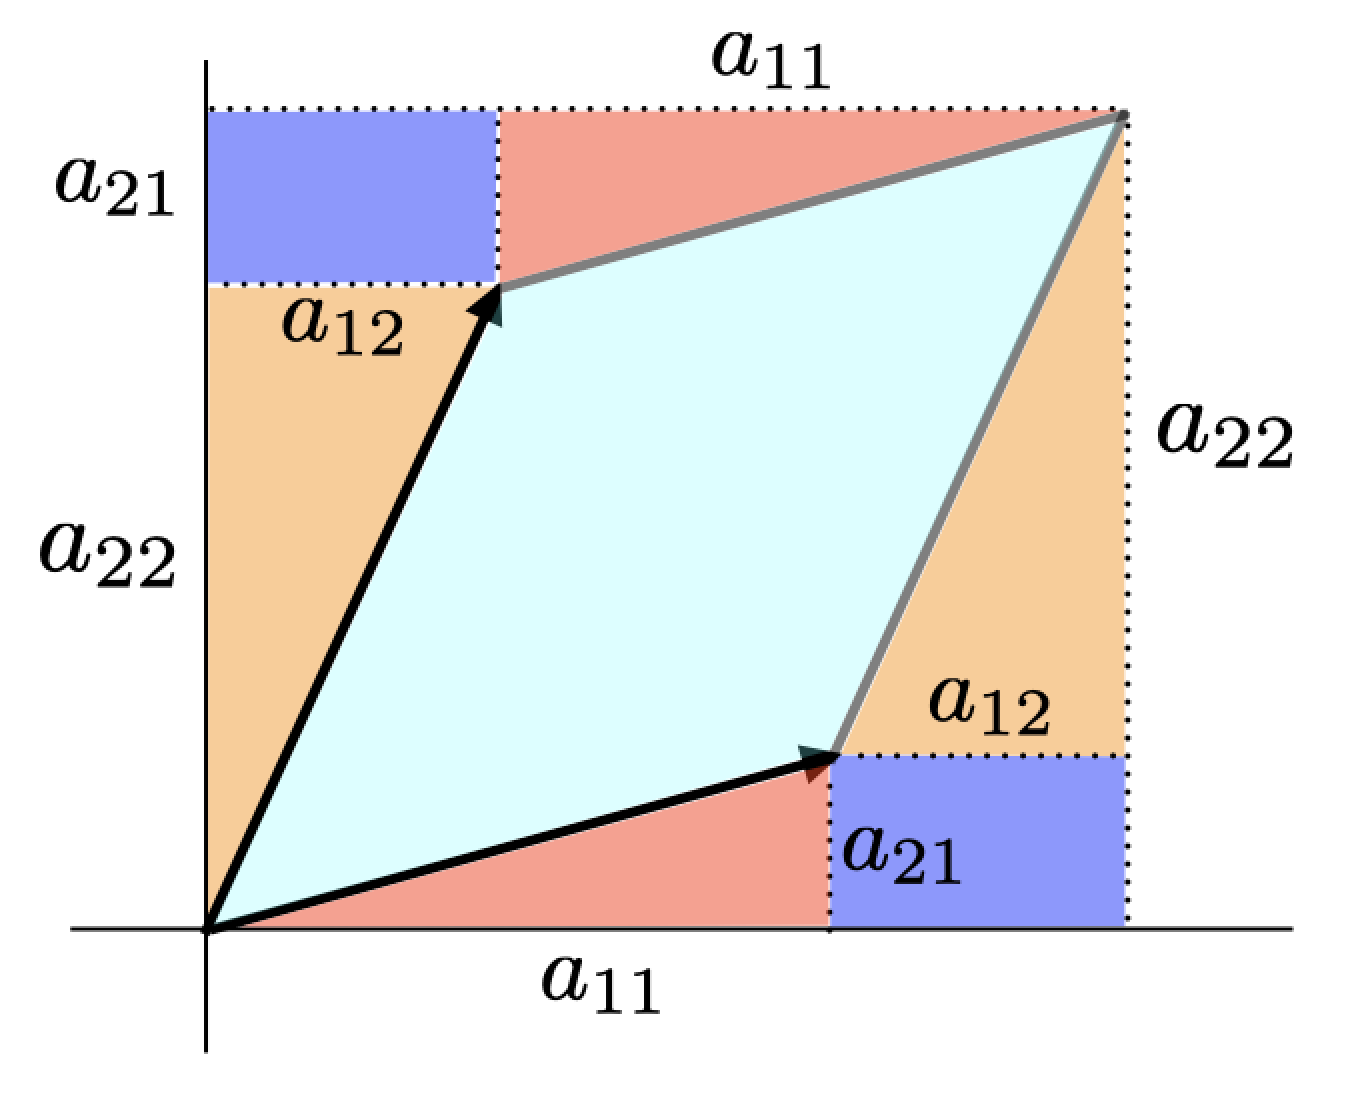
\includegraphics[width = 0.4\textwidth]{media/determinanteFlaeche2.png}
        \end{center}
      \end{enumerate}
      
  \end{LA}
  \clearpage
  Die Erkenntnisse aus \Cref{LA:determinanteUndFläche} gelten aufgrund der Linearität nicht nur für das Einheitsquadrat:
  \begin{satz}
    {Bedeutung der Determinante}{}
    Sei $f$ eine lineare Abbildung mit der Abbildungsmatrix $A$. Wird eine Figur mit dem Flächeninhalt $I$ abgebildet so hat die Bildfigur den Flächeninhalt

    $$ I' = |\det(A)| \cdot I$$
  \end{satz}

  \begin{ueb}
    {}{}
    \begin{enumerate}
        \item Welchen Wert hat die Determinante der Abbildung aufgrund der geometrischen Interpretation? Überprüfe die Vermutung, indem du die zur Abbildung passende Matrix bestimmst und deren Determinante berechnest
         \begin{enumerate}
            \item Drehung um den Ursprung um den Winkel \( \alpha \).
            \item Zentrische Streckung um den Faktor 5 mit Zentrum im Ursprung. 
            \item Projektion auf die \( y \)-Achse in Richtung des Vektors \( \vec{v} = \begin{pmatrix} 2 \\ 5 \end{pmatrix} \)
          \end{enumerate}
        \item Seien $A$ und $B$ $2\times2$-Matrizen und $\lambda\in\R$ eine Zahl. Welche Beziehung besteht zwischen 
        \begin{enumerate}
            \item $\det(A)$ und $\det(\lambda\cdot A)$?
            \item $\det(A), \det(B)$ und $\det(AB)$?
        \end{enumerate}
        Beweise die Vermutungen mit einer Rechnung.
    \end{enumerate}
  \end{ueb}
  

























  \clearpage
  \subsection{Lineare Gleichungssysteme und Matrizen}

Matrizen haben viel mit linearen Gleichungssystemen zu tun. Tatsächlich kann man jedes lineare Gleichungssystem mithilfe von Matrizen beschreiben und auch lösen.

Betrachten Sie das folgende Beispiel:

\begin{bsp}
    {Gleichungssystem in Matrixform}{}

\[
\begin{cases}
2x + 2y = -2 \\
5x + 6y = 6
\end{cases}
\]

Dieses Gleichungssystem kann auch in Matrixform geschrieben werden:

\vspace*{15cm}

% \[
% \begin{pmatrix}
% 2 & 2 \\
% 5 & 6
% \end{pmatrix}
% \cdot
% \begin{pmatrix}
% x \\
% y
% \end{pmatrix}
% =
% \begin{pmatrix}
% -2 \\
% 6
% \end{pmatrix}
% \]

% Unter diesem Blickwinkel wird nach einem Vektor $\begin{pmatrix}
%     x \\
%     y
%     \end{pmatrix}$ gesucht, der auf den Vektor $\begin{pmatrix}
%         -2 \\
%         6
%         \end{pmatrix}$ abgebildet wird. Für diese Fragestellung kennen wir bereits einen Lösungsweg:

% Die Inverse der Matrix \( A = \begin{pmatrix} 2 & 2 \\ 5 & 6 \end{pmatrix} \) ist:

% \[
% A^{-1} = \frac{1}{2} \begin{pmatrix} 6 & -2 \\ -5 & 2 \end{pmatrix}
% \]

% Daraus folgt:

% \[
% \begin{pmatrix}
% x \\
% y
% \end{pmatrix}
% =
% A^{-1} \cdot
% \begin{pmatrix}
% -2 \\
% 6
% \end{pmatrix}
% =
% \begin{pmatrix}
% -12 \\
% 11
% \end{pmatrix}
% \]

% Das Gleichungssystem hat also die Lösung \( x = -12 \), \( y = 11 \).
\end{bsp}
\clearpage
\begin{satz}
    {Matrizen und lineare Gleichungssysteme}{}
    Für das lineare Gleichungssystem
\[
\begin{cases}
a_{11}x + a_{12}y = b_1 \\
a_{21}x + a_{22}y = b_2
\end{cases}
\]
und die zugehörige Koeffizientenmatrix
\[
A = \begin{pmatrix}
a_{11} & a_{12} \\
a_{21} & a_{22}
\end{pmatrix}
\]
gilt:

\begin{itemize}
  \item Falls \( \det(A) \neq 0 \), so hat das Gleichungssystem genau eine Lösung, nämlich:
  \[
  \begin{pmatrix}
  x \\
  y
  \end{pmatrix}
  = A^{-1} \cdot
  \begin{pmatrix}
  b_1 \\
  b_2
  \end{pmatrix}
  \]
  
  \item Falls \( \det(A) = 0 \), so hat das Gleichungssystem entweder keine Lösung oder unendlich viele Lösungen.
\end{itemize}
\end{satz}
\paragraph{Bemerkung:}
Diese Lösungsmethode kann auch verwendet werden, um lineare Gleichungssysteme mit drei und mehr Unbekannten zu lösen (vorausgesetzt, es liegen entsprechend viele Gleichungen vor). 
Allerdings ist bereits ab drei Unbekannten der Aufwand zur Ermittlung der inversen Matrix so gross, dass sich die Lösung mit anderen Methoden — zum Beispiel dem Gauss-Verfahren — effizienter finden lässt.

\begin{ueb}
    {}{}

\begin{enumerate}
    \item Lösen Sie die folgenden Gleichungssysteme mit Hilfe der inversen Matrix:
    \begin{enumerate}
      \item
      \[
      \begin{cases}
      3x + 2y = -2 \\
      7x + 5y = 3
      \end{cases}
      \]
      \item
      \[
      \begin{cases}
      x + y = 26 \\
      x - y = 8
      \end{cases}
      \]
      \item
      \[
      \begin{cases}
      3x + 4y = 24 \\
      -x + 5y = 11
      \end{cases}
      \]
      \item
      \[
      \begin{cases}
      8x + 5y - 7 = 0 \\
      4x + 3y - 1 = 0
      \end{cases}
      \]
      \item
      \[
      \begin{cases}
      -4x + 6y = 5 \\
      6x - 9y = -8
      \end{cases}
      \]
      \item
      \[
      \begin{cases}
      -4x + 6y = 5 \\
      6x - 9y = -7.5
      \end{cases}
      \]
    \end{enumerate}
  
    \item Für welche Werte des Parameters besitzt das Gleichungssystem eine eindeutige Lösung?\\
    Begründen Sie, indem Sie die Determinante der entsprechenden Matrix untersuchen.
    \begin{enumerate}
      \item
      \[
      \begin{cases}
      ax + y = 5 \\
      x - y = -8
      \end{cases}
      \]
      \item
      \[
      \begin{cases}
      bx + by = 5 \\
      6x + by = -8
      \end{cases}
      \]
      \item
      \[
      \begin{cases}
      3x + 3cy = 5 \\
      cx + x + 3y = -8
      \end{cases}
      \]
    \end{enumerate}
  \end{enumerate}
  
\end{ueb}
\clearpage
\emph{Lösungen}

\begin{enumerate}
    \item Lösungen der Gleichungssysteme mit der inversen Matrix:
    \begin{enumerate}
      \item \( x = -16, \quad y = 23 \)
      \item \( x = 17, \quad y = 9 \)
      \item \( x = 4, \quad y = 3 \)
      \item \( x = 4, \quad y = -5 \)
      \item Keine Lösung .
      \item Unendlich viele Lösungen  
      Parametrisierte Lösungsmenge:
      \[
      \begin{pmatrix}
      x \\
      y
      \end{pmatrix}
      =
      \begin{pmatrix}
      -5 \\
      -\frac{5}{2}
      \end{pmatrix}
      +
      t \cdot
      \begin{pmatrix}
      \frac{3}{2} \\
      1
      \end{pmatrix},
      \quad t \in \mathbb{R}
      \]
    \end{enumerate}
    
  \item Eindeutige Lösbarkeit in Abhängigkeit vom Parameter:
  \begin{enumerate}
    \item Eindeutig lösbar für \( a \neq 1 \)
    \item Eindeutig lösbar für \( b \neq 0 \) und $b\neq 6$
    \item Eindeutig lösbar für \( c \neq -\frac{1}{2} \pm \frac{\sqrt{13}}{2} \)
  \end{enumerate}
  \end{enumerate}
\clearpage
\subsection{LGS mit nicht-invertierbarer Matrix}

Im vorangegangenen Abschnitt haben wir gesehen, dass man Gleichungssysteme leicht mit Hilfe der inversen Matrix lösen kann. In diesem Kapitel wollen wir den Fall untersuchen, dass die Matrix nicht invertierbar ist. 

\begin{LA}
{}{}
In dieser Lernaufgabe untersuchen wir Gleichungssysteme der Form
$$ A\cdot \begin{pmatrix}
    x\\y
\end{pmatrix}= \vec{b} \qquad \text{ bzw. } \qquad B\cdot \begin{pmatrix}
    x\\y
\end{pmatrix}= \vec{b}$$
mit den (nicht invertierbaren) Matrizen
$$ A = \begin{pmatrix}
    4 & -6\\
    -6 & 9
\end{pmatrix} \qquad \text{ bzw. } \qquad B = \begin{pmatrix}
    12 & 20\\
    9 & 15
\end{pmatrix}$$


\textbf{Teil 1}: der Kern der Matrix

\begin{enumerate}
    \item Finden Sie drei Lösungen der Gleichung $A\cdot \begin{pmatrix}
    x\\y
\end{pmatrix}= \begin{pmatrix}
    0\\0
\end{pmatrix}$
\item Zeigen Sie, dass die drei Lösungen alle auf einer Geraden liegen und diese Gerade der Menge $\left\{t\cdot \begin{pmatrix}
    3\\2
\end{pmatrix} \mid t \in \R\right\}$ entspricht.
\item Betrachten Sie nun die Matrix $B$. Bestimmen die Lösungsmenge der Gleichung $B\cdot \begin{pmatrix}
    x\\y
\end{pmatrix}= \begin{pmatrix}
    0\\0
\end{pmatrix}$.
\end{enumerate}

\textbf{Teil 2:} das Bild der Matrix
\begin{enumerate}
    \item Berechnen Sie $A \cdot \vec{v}$ für drei verschiedene Vektoren $\vec{v} \in \R^2$.
    \item Zeigen Sie, dass die drei Vektoren $A \cdot \vec{v}$ alle auf einer Geraden liegen und diese Gerade der Menge $\left\{t\cdot \begin{pmatrix}
    2\\-3
\end{pmatrix} \mid t \in \R\right\}$ entspricht.
    \item Betrachten Sie nun die Matrix $B$. Bestimmen Sie die Menge aller Bilder $B \cdot \vec{v}$ für $\vec{v} \in \R^2$.

\end{enumerate}

\textbf{Teil 3:}
\begin{enumerate}
    \item Erklären Sie in Bezugnahme auf `Teil 2', wieso das Gleichungssystem 
    $$A\cdot \begin{pmatrix}
    x\\y
\end{pmatrix}= \begin{pmatrix}
    10\\10
\end{pmatrix}$$
keine Lösung hat.
\item Der Vektor $\begin{pmatrix}
    5\\-2
\end{pmatrix}$ ist eine Lösung des Gleichungssystems
$$A\cdot \begin{pmatrix}
    x\\y
\end{pmatrix}= \begin{pmatrix}
    32\\-48
\end{pmatrix}$$
Erklären Sie in Bezugnahme auf `Teil 1', wieso jeder Vektor der Form
$$\begin{pmatrix}
    5\\-2
\end{pmatrix} + t \cdot \begin{pmatrix}
    3\\2
\end{pmatrix}$$
mit $t \in \R$ eine Lösung des Gleichungssystems ist.
\end{enumerate}

\textbf{Teil 4:}

Entscheiden Sie, ob die folgenden Gleichungssysteme Lösungen haben und wenn ja, geben Sie die Lösungsmenge an.
\begin{enumerate}
    \item $B \cdot \begin{pmatrix}
    x\\y
\end{pmatrix}= \begin{pmatrix}
    6\\8
\end{pmatrix}$
    \item $B \cdot \begin{pmatrix}
    x\\y
\end{pmatrix}= \begin{pmatrix}
    8\\6
\end{pmatrix}$
\end{enumerate}
\end{LA}





















\clearpage
Im folgenden werden einige neue Begriffe eingeführt, mit denen man die Lösungsmenge eines LGS mit nicht-invertierbarer Matrix beschreiben kann. Diese Begriffe sind wichtig, um die Lösungsmenge eines LGS zu verstehen und zu beschreiben.

\begin{definition}
    {Kern und Bild}{}
   
Sei \( A\) eine $2\times2$-Matrix. 

Die Menge aller Vektoren, die auf den Nullvektor abgebildet werden, nennt man den \emph{Kern} von \( A \) und schreibt dafür:
\[
\ker(A) = \left\{ \vec{v} \in \mathbb{R}^2 \mid A\cdot \vec{v} = \vec{0} \right\}
\]

Die Menge aller Bilder $A\cdot \vec{v}$ von \( A \) nennt man das \emph{Bild} von \( A \) und schreibt dafür:
\[
\operatorname{im}(f) = \left\{ A\cdot \vec{v} \mid \vec{v} \in \mathbb{R}^2 \right\}
\]
Die Bezeichnung \( \operatorname{im} \) steht für \emph{image} (englisch für Bild).


\end{definition}


\begin{bsp}
    {Kern und Bild von $A = \begin{pmatrix} 1 & 3 \\ 3 & 9 \end{pmatrix}$ }{}


Dreimal die erste Spalte minus die zweite ergibt den Nullvektor, also ist:
\[
\ker(A) = \left\{ t \begin{pmatrix} 3 \\ -1 \end{pmatrix} \;\middle|\; t \in \mathbb{R} \right\}.
\]

Beide Spalten sind Vielfache des Vektors $\begin{pmatrix} 1 \\ 3 \end{pmatrix}$.  
Also gilt:
\[
\operatorname{im}(A) = \left\{ t \begin{pmatrix} 1 \\ 3 \end{pmatrix} \;\middle|\; t \in \mathbb{R} \right\}.
\]

\end{bsp}

\begin{bsp}
{Kern und Bild von $B = \begin{pmatrix} 1 & 3 \\ 4 & -1 \end{pmatrix}.$}{}

Die Matrix ist invertierbar, weil $\det(B)  = -13 \neq 0$. 
Also gilt:

\[
\ker(B) = \left\{B^{-1}\cdot \vec{0} \right\} = \left\{ \vec{0} \right\}.
\]
und 
\[
\operatorname{im}(B)  = \mathbb{R}^2.
\]

\end{bsp}

\begin{bsp}
{Kern und Bild von $N = \begin{pmatrix} 0 & 0 \\ 0 & 0 \end{pmatrix}.$}{}

Die Matrix $N$ bildet jeden Vektor auf den Nullvektor ab.
Also gilt:
\[
\ker(N) = \R^2.
\]
und 
\[
\operatorname{im}(N)  = \left\{\vec{0}\right\}.
\]

\end{bsp}

Mit diesen Begriffen kann man die Lösungsmenge eines LGS mit nicht-invertierbarer Matrix beschreiben.
\begin{satz}{Lösung von LGS }{}
Sei \( A \) eine $2\times2$-Matrix und \( \vec{b} \in \mathbb{R}^2 \). Dann gilt:
\begin{itemize}
    \item Falls $A$ invertierbar ist, dann hat das LGS \( A\cdot \vec{x} = \vec{b} \) genau eine Lösung, nämlich \( \vec{x} = A^{-1}\cdot \vec{b} \).
    \item Falls $A$ nicht invertierbar ist, dann gilt:
\begin{itemize}
    \item Wenn \( \vec{b} \notin \operatorname{im}(A) \), dann hat das LGS \( A\cdot \vec{x} = \vec{b} \) keine Lösung.
    \item Wenn \( \vec{b} \in \operatorname{im}(A) \), dann hat das LGS \( A\cdot \vec{x} = \vec{b} \) unendlich viele Lösungen. 
    \item Ist \( \vec{x}_0 \) eine Lösung des LGS \( A\cdot \vec{x} = \vec{b} \), dann ist die Menge aller Lösungen gegeben durch:
    \[
    \left\{ \vec{x}_0 + \vec{v} \mid \vec{v} \in \ker(A) \right\}.
    \]
\end{itemize}
\end{itemize}
\end{satz}

\begin{bsp}
{ $ \begin{pmatrix} 1 & 3 \\ 3 & 9 \end{pmatrix} \cdot \vec{x} = \begin{pmatrix}
    8\\ 16
\end{pmatrix}$ }{}

\vspace*{7 cm}
% Sei $A = \begin{pmatrix} 1 & 3 \\ 3 & 9 \end{pmatrix} $. 
% Das Bild von $A$ ist die Gerade durch den Nullvektor in Richtung $\begin{pmatrix} 1 \\ 3 \end{pmatrix}$.
% Der Vektor $\begin{pmatrix} 8 \\ 16 \end{pmatrix}$ liegt nicht auf dieser Geraden, also hat das LGS keine Lösung.
\end{bsp}

\begin{bsp}
{$\begin{pmatrix} 1 & 3 \\ 3 & 9 \end{pmatrix} \cdot \vec{x} = \begin{pmatrix}
    8\\ 24
\end{pmatrix}$ }{}

\vspace*{12 cm}

% Sei wieder $A = \begin{pmatrix} 1 & 3 \\ 3 & 9 \end{pmatrix} $. 
% Der Vektor $\begin{pmatrix} 8 \\ 24 \end{pmatrix}$ liegt im Bild von $A$. 

% Der Kern von $A$ ist gegeben durch:
% \[
% \ker(A) = \left\{ t \begin{pmatrix} 3 \\ -1 \end{pmatrix} \;\middle|\; t \in \mathbb{R} \right\}.
% \]


% Eine Lösung des LGS ist $\begin{pmatrix} 2 \\ 2 \end{pmatrix}$.

% Die gesamte Lösungsmenge ist gegeben durch:
% \[
% \left\{ \begin{pmatrix} 2 \\ 2 \end{pmatrix} + t \begin{pmatrix} 3 \\ -1 \end{pmatrix} \;\middle|\; t \in \mathbb{R} \right\}.
% \]
\end{bsp}

\clearpage

\begin{ueb}
    {}{}

\begin{enumerate}
  \item Bestimmen Sie den Kern und das Bild der folgenden Matrizen.  
  \begin{enumerate}
    \item \( A = \begin{pmatrix} 1 & 2 \\ 3 & 4 \end{pmatrix} \)
    \item \( B = \begin{pmatrix} 0 & 0 \\ 0 & 0 \end{pmatrix} \)
    \item \( C = \begin{pmatrix} 2 & 12 \\ -1 & -6 \end{pmatrix} \)
    \item \( D = \begin{pmatrix} -6 & 7 \\ 12 & -14 \end{pmatrix} \)
    \item \( E = \begin{pmatrix} 1 & 3 \\ 0 & 0 \end{pmatrix} \)
  \end{enumerate}

  \item Geben Sie die Lösungsmenge der folgenden LGS an. Die Matrizen beziehen sich auf die Aufgabe 1.
  \begin{enumerate}
    \item \( A \cdot \begin{pmatrix} x \\ y \end{pmatrix} = \begin{pmatrix} 1 \\ 2 \end{pmatrix} \)
    \item  \( B \cdot \begin{pmatrix} x \\ y \end{pmatrix} = \begin{pmatrix} 0 \\ 0 \end{pmatrix} \)
    \item \( C \cdot \begin{pmatrix} x \\ y \end{pmatrix} = \begin{pmatrix} 3 \\ 20 \end{pmatrix} \)
    \item \( D \cdot \begin{pmatrix} x \\ y \end{pmatrix} = \begin{pmatrix} -5 \\ 10 \end{pmatrix} \)
    \item \( E \cdot \begin{pmatrix} x \\ y \end{pmatrix} = \begin{pmatrix} 1 \\ 0 \end{pmatrix} \)
  \end{enumerate}

  \item Sei \( f \) die Projektion auf die Gerade \( y = x \) in Richtung  
  \( \vec{v} = \begin{pmatrix} 1 \\ -1 \end{pmatrix} \).  
  Bestimmen Sie den Kern und das Bild von \( f \).

  \item Geben Sie eine Matrix an, deren Kern die Gerade  
  \( g \colon \vec{r}(t) = t \begin{pmatrix} 1 \\ 2 \end{pmatrix} \)  
  und deren Bild die \( y \)-Achse ist.

  \item Geben Sie eine Matrix \( A \) an, deren Kern und Bild übereinstimmen.  
  Was ergibt \( A^2 \)?

  \item Sei \( f \) die Spiegelung an der \( xz \)-Ebene.  
  Bestimmen Sie den Kern und das Bild.

  \item Sei \( f \) die orthogonale Projektion auf die \( xz \)-Ebene.  
  Bestimmen Sie den Kern und das Bild.

  \item \textbf{Challenge:}
  
    Beweisen Sie die folgende Aussage:  
    Sei \( f \) eine lineare Abbildung mit \( \ker(f) = \{ \vec{0} \} \).  
    Dann ist \( f \) injektiv.\\
    \emph{Tipp:} Injektiv bedeutet: Aus \( f(\vec{v}) = f(\vec{w}) \) folgt \( \vec{v} = \vec{w} \).  
    Betrachten Sie \( f(\vec{v} - \vec{w}) \).

\end{enumerate}

\end{ueb}

\clearpage
\emph{Lösungen:}
\begin{enumerate}
  \item 
  \begin{enumerate}
    \item \( \ker(A) = \left\{ \vec{0} \right\} \), \( \operatorname{im}(A) = \mathbb{R}^2 \)
    \item \( \ker(B) = \mathbb{R}^2 \), \( \operatorname{im}(B) = \left\{ \vec{0} \right\} \)
    \item \( \ker(C) = \left\{ t\begin{pmatrix} 6 \\ -1 \end{pmatrix} | t\in\mathbb{R}  \right\}  ,  \operatorname{im}(C) =  \left\{ t\begin{pmatrix} 2 \\ -1  \end{pmatrix} | t\in\mathbb{R}  \right\}\)
    \item \( \ker(D) = \left\{ t\begin{pmatrix} 7 \\ 6 \end{pmatrix} | t\in\mathbb{R}  \right\}  ,  \operatorname{im}(D) =  \left\{ t\begin{pmatrix} -1 \\ 2  \end{pmatrix} | t\in\mathbb{R}  \right\}\)
    \item \( \ker(E) = \left\{ t\begin{pmatrix} 3 \\ -1 \end{pmatrix} | t\in\mathbb{R}  \right\}  ,  \operatorname{im}(E) =  \left\{ t\begin{pmatrix} 1 \\ 0  \end{pmatrix} | t\in\mathbb{R}  \right\}\)
    \end{enumerate}
    \item \begin{enumerate}
        \item $\LL = \left\{\begin{pmatrix}
            0 \\ \frac{1}{2}
        \end{pmatrix}\right\}$
        \item $\LL = \R^2$
        \item $\LL = \emptyset$
        \item $\LL = \left\{\begin{pmatrix}
            \frac{5}{6} \\ 0
        \end{pmatrix} + t\begin{pmatrix}
            7 \\ 6
        \end{pmatrix} \mid t \in \R\right\}$
        \item $\LL = \left\{\begin{pmatrix}
            1 \\ 0
        \end{pmatrix} + t\begin{pmatrix}
            3 \\ -1
        \end{pmatrix} \mid t \in \R\right\}$
    \end{enumerate}
    \item \( \ker(f) = \left\{ t \begin{pmatrix} 1 \\ -1 \end{pmatrix} \;\middle|\; t \in \mathbb{R} \right\} \) und $\operatorname{im}(f) = \left\{ t \begin{pmatrix} 1 \\ 1 \end{pmatrix} \;\middle|\; t \in \mathbb{R} \right\}$.
    \item Z.B. \( \begin{pmatrix} 0 & 0 \\ 2 & -1 \end{pmatrix} \)
    \item Z.B. \( \begin{pmatrix} 0 & 0 \\  1 & 0\end{pmatrix} \). Dann ist logischerweise $A^2 = \begin{pmatrix} 0 & 0 \\  0 & 0\end{pmatrix}$.
    \item \( \ker(f) = \left\{ \vec{0} \right\} \) und \( \operatorname{im}(f) = \R^3 \)
    \item \( \ker(f) = \left\{ \begin{pmatrix} 0 \\ y \\ 0 \end{pmatrix} \;\middle|\; y \in \mathbb{R} \right\} \) und \( \operatorname{im}(f) = \left\{ \begin{pmatrix} x \\ 0 \\ z \end{pmatrix} \;\middle|\; x,z \in \mathbb{R} \right\} \)
\end{enumerate}



\end{document}